\chapter{Gültigkeit}
\label{kap:5}
\bookmarksetupnext{level=subsubsection}
\chapterinfo{Die entscheidenden Versuchsparameter werden durch selbstgebaute Apparaturen gemessen und mit den theoretischen Erwartungen verglichen, um aus der Schnittmenge ein mathematisches Modell des Analogieexperimentes zu entwickeln.}

\textit{Die entscheidenden Versuchsparameter werden durch selbstgebaute Apparaturen gemessen und mit den theoretischen Erwartungen verglichen, um aus der Schnittmenge ein mathematisches Modell des Analogieexperimentes zu entwickeln.}

\section{Kraftmessung im Strömungsfeld}

Mit dem Ziel, die Krafteinwirkung des Gebläses auf vorbeirollende Kugeln --- und damit auch die Impulsänderung --- funktional ausdrücken zu können, wird eine Methode erarbeitet, das Strömungsfeld des Föhns systematisch zu vermessen.

Zuerst wird, da Luftwiderstandsbeiwerte zumeist mit einem \textit{Sektor-Kraftmesser} bestimmt werden, der Versuch unternommen, diese Art von Messgerät nachzubauen. Das Prinzip eines Sektor-Kraftmessers kann mit einem Messwagen, der auf einem Gleis positioniert und über eine Umlenkrolle mit einem Federkraftmesser verbunden ist, imitiert werden.

%% Autor: Björn Ritterbecks 
%% Letzte Aenderung: 15.06.2016 
\thisfloatsetup{%
  capbesidewidth=\marginparwidth,}
\begin{figure}[htbp]
\centering
%\sansmath
\begin{tikzpicture}[      
        every node/.style={anchor=south west,inner sep=0pt},
        x=1mm, y=1mm,
      ]   
     \node (fig1) at (0,0)
       {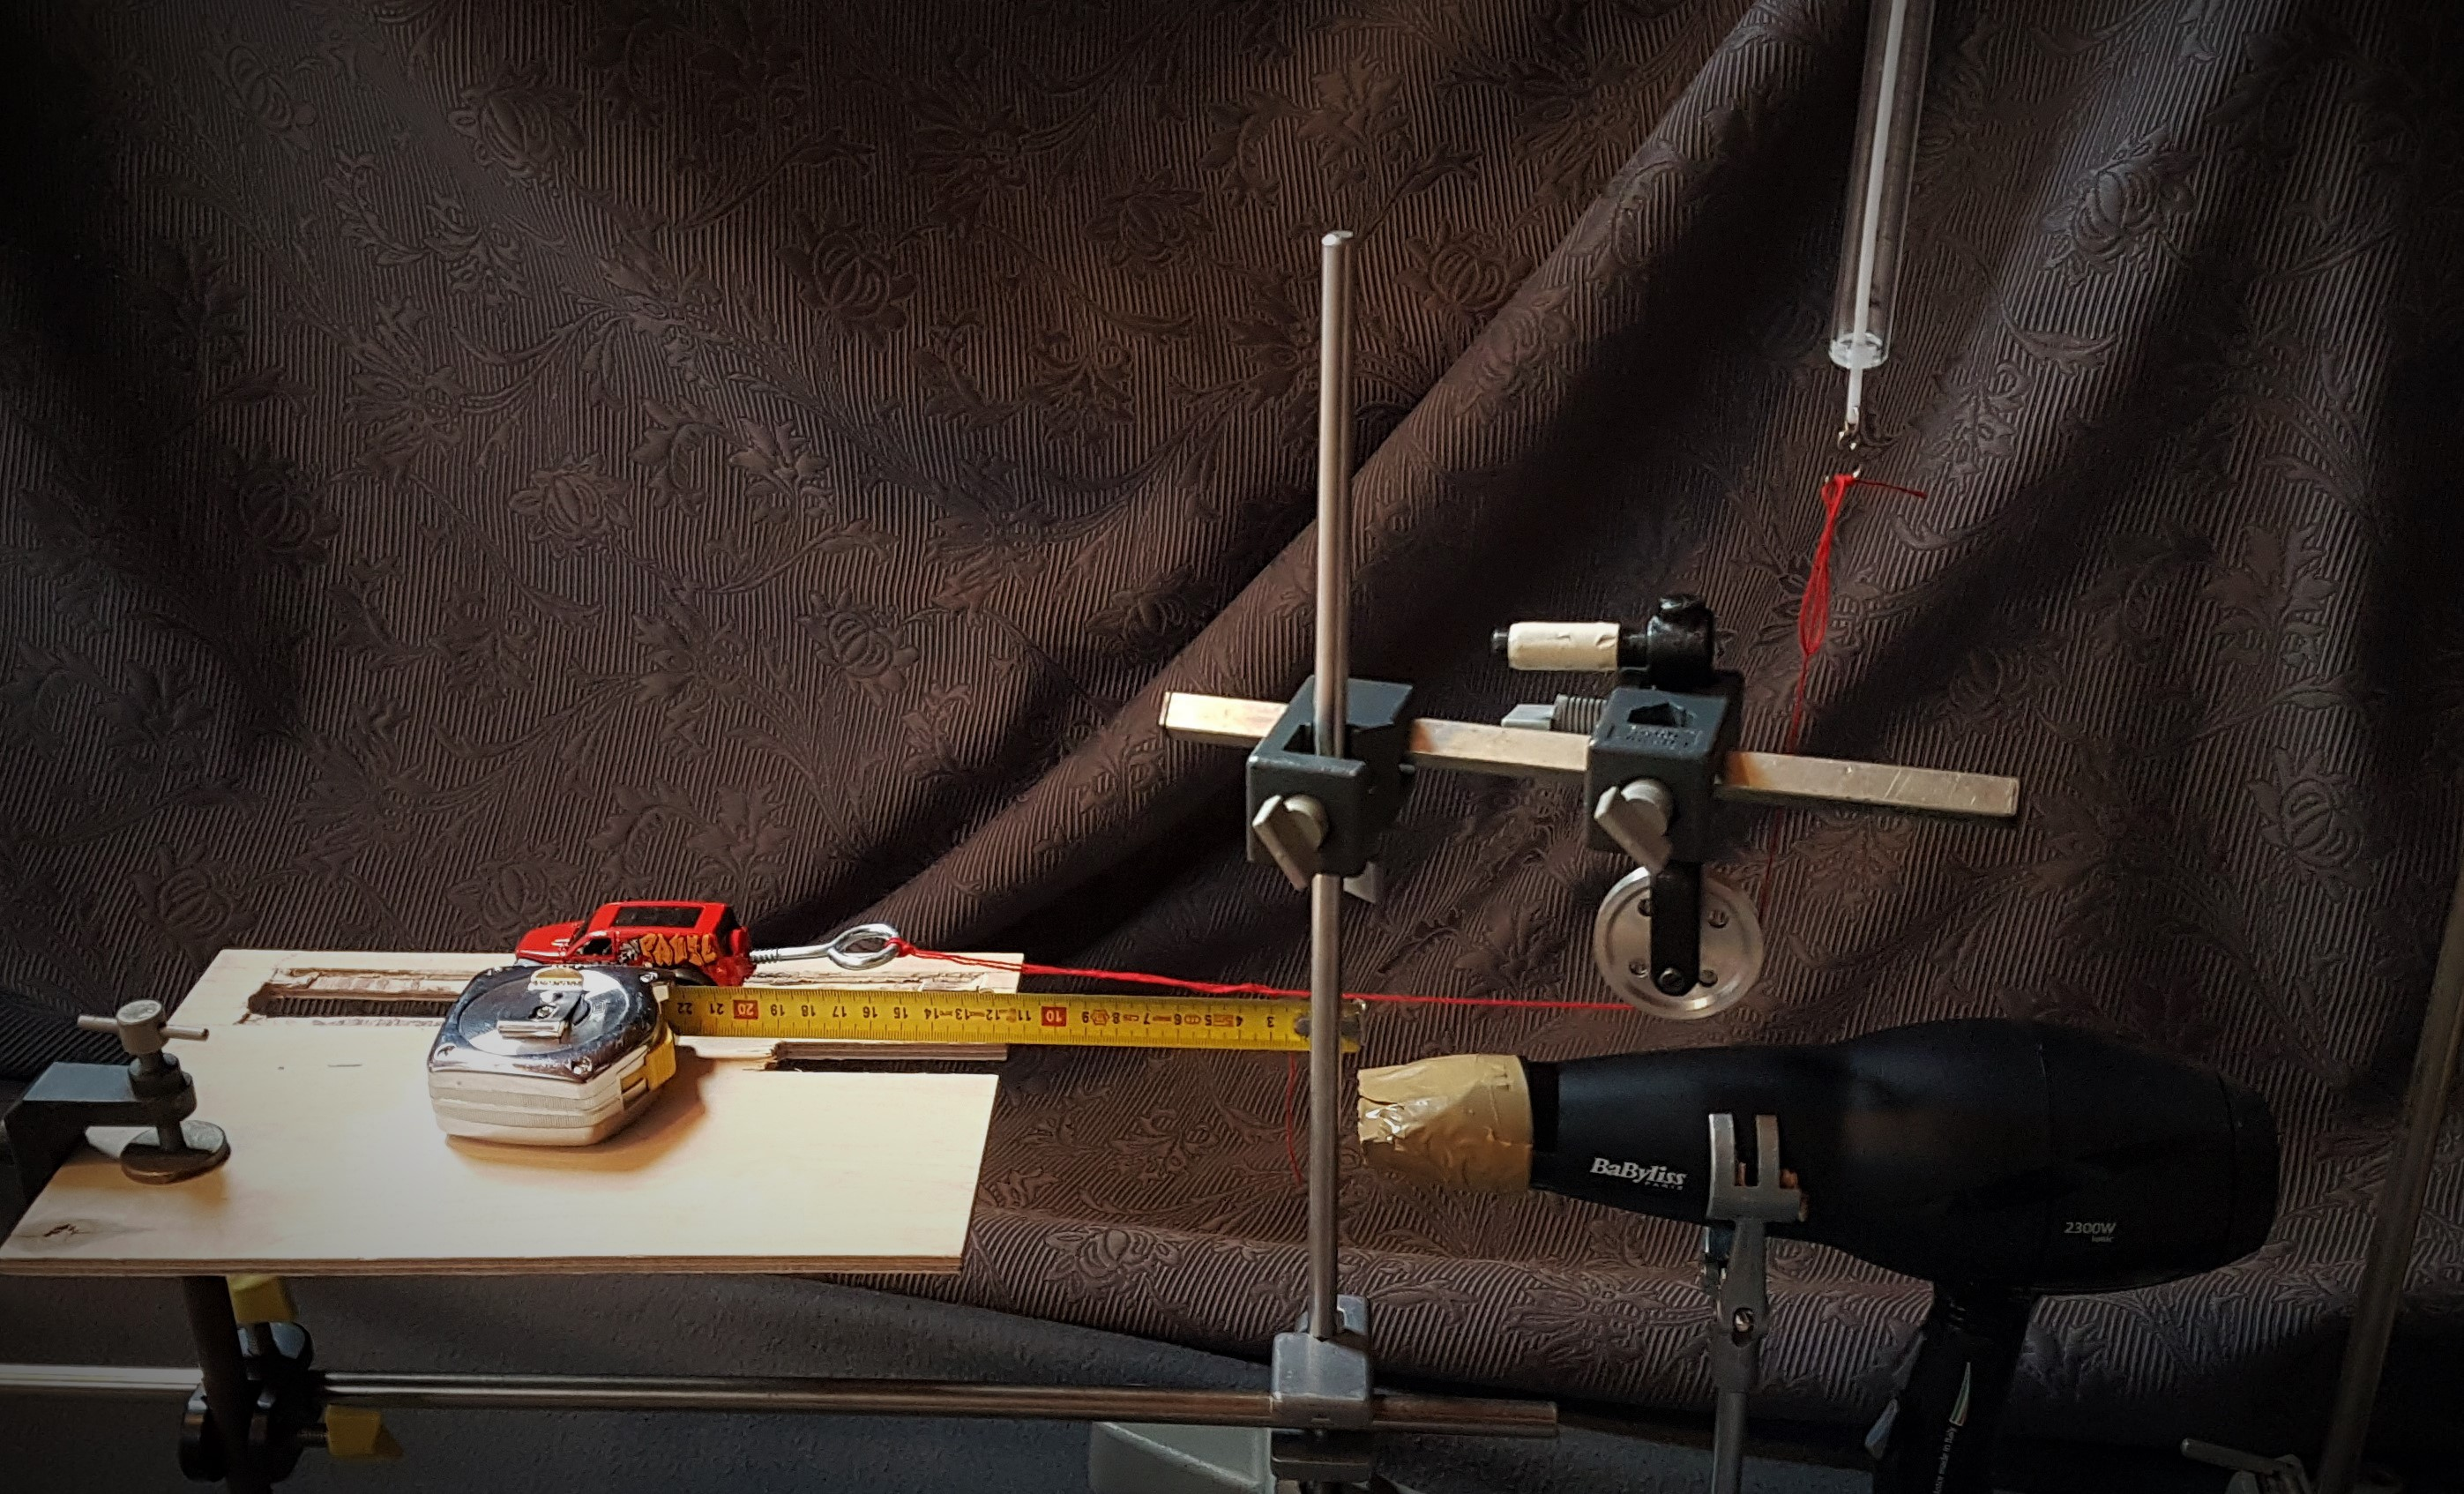
\includegraphics[scale=0.108]{images/stroemungskraftmessung1.jpg}};
     \node (fig2) at (3,40)
       {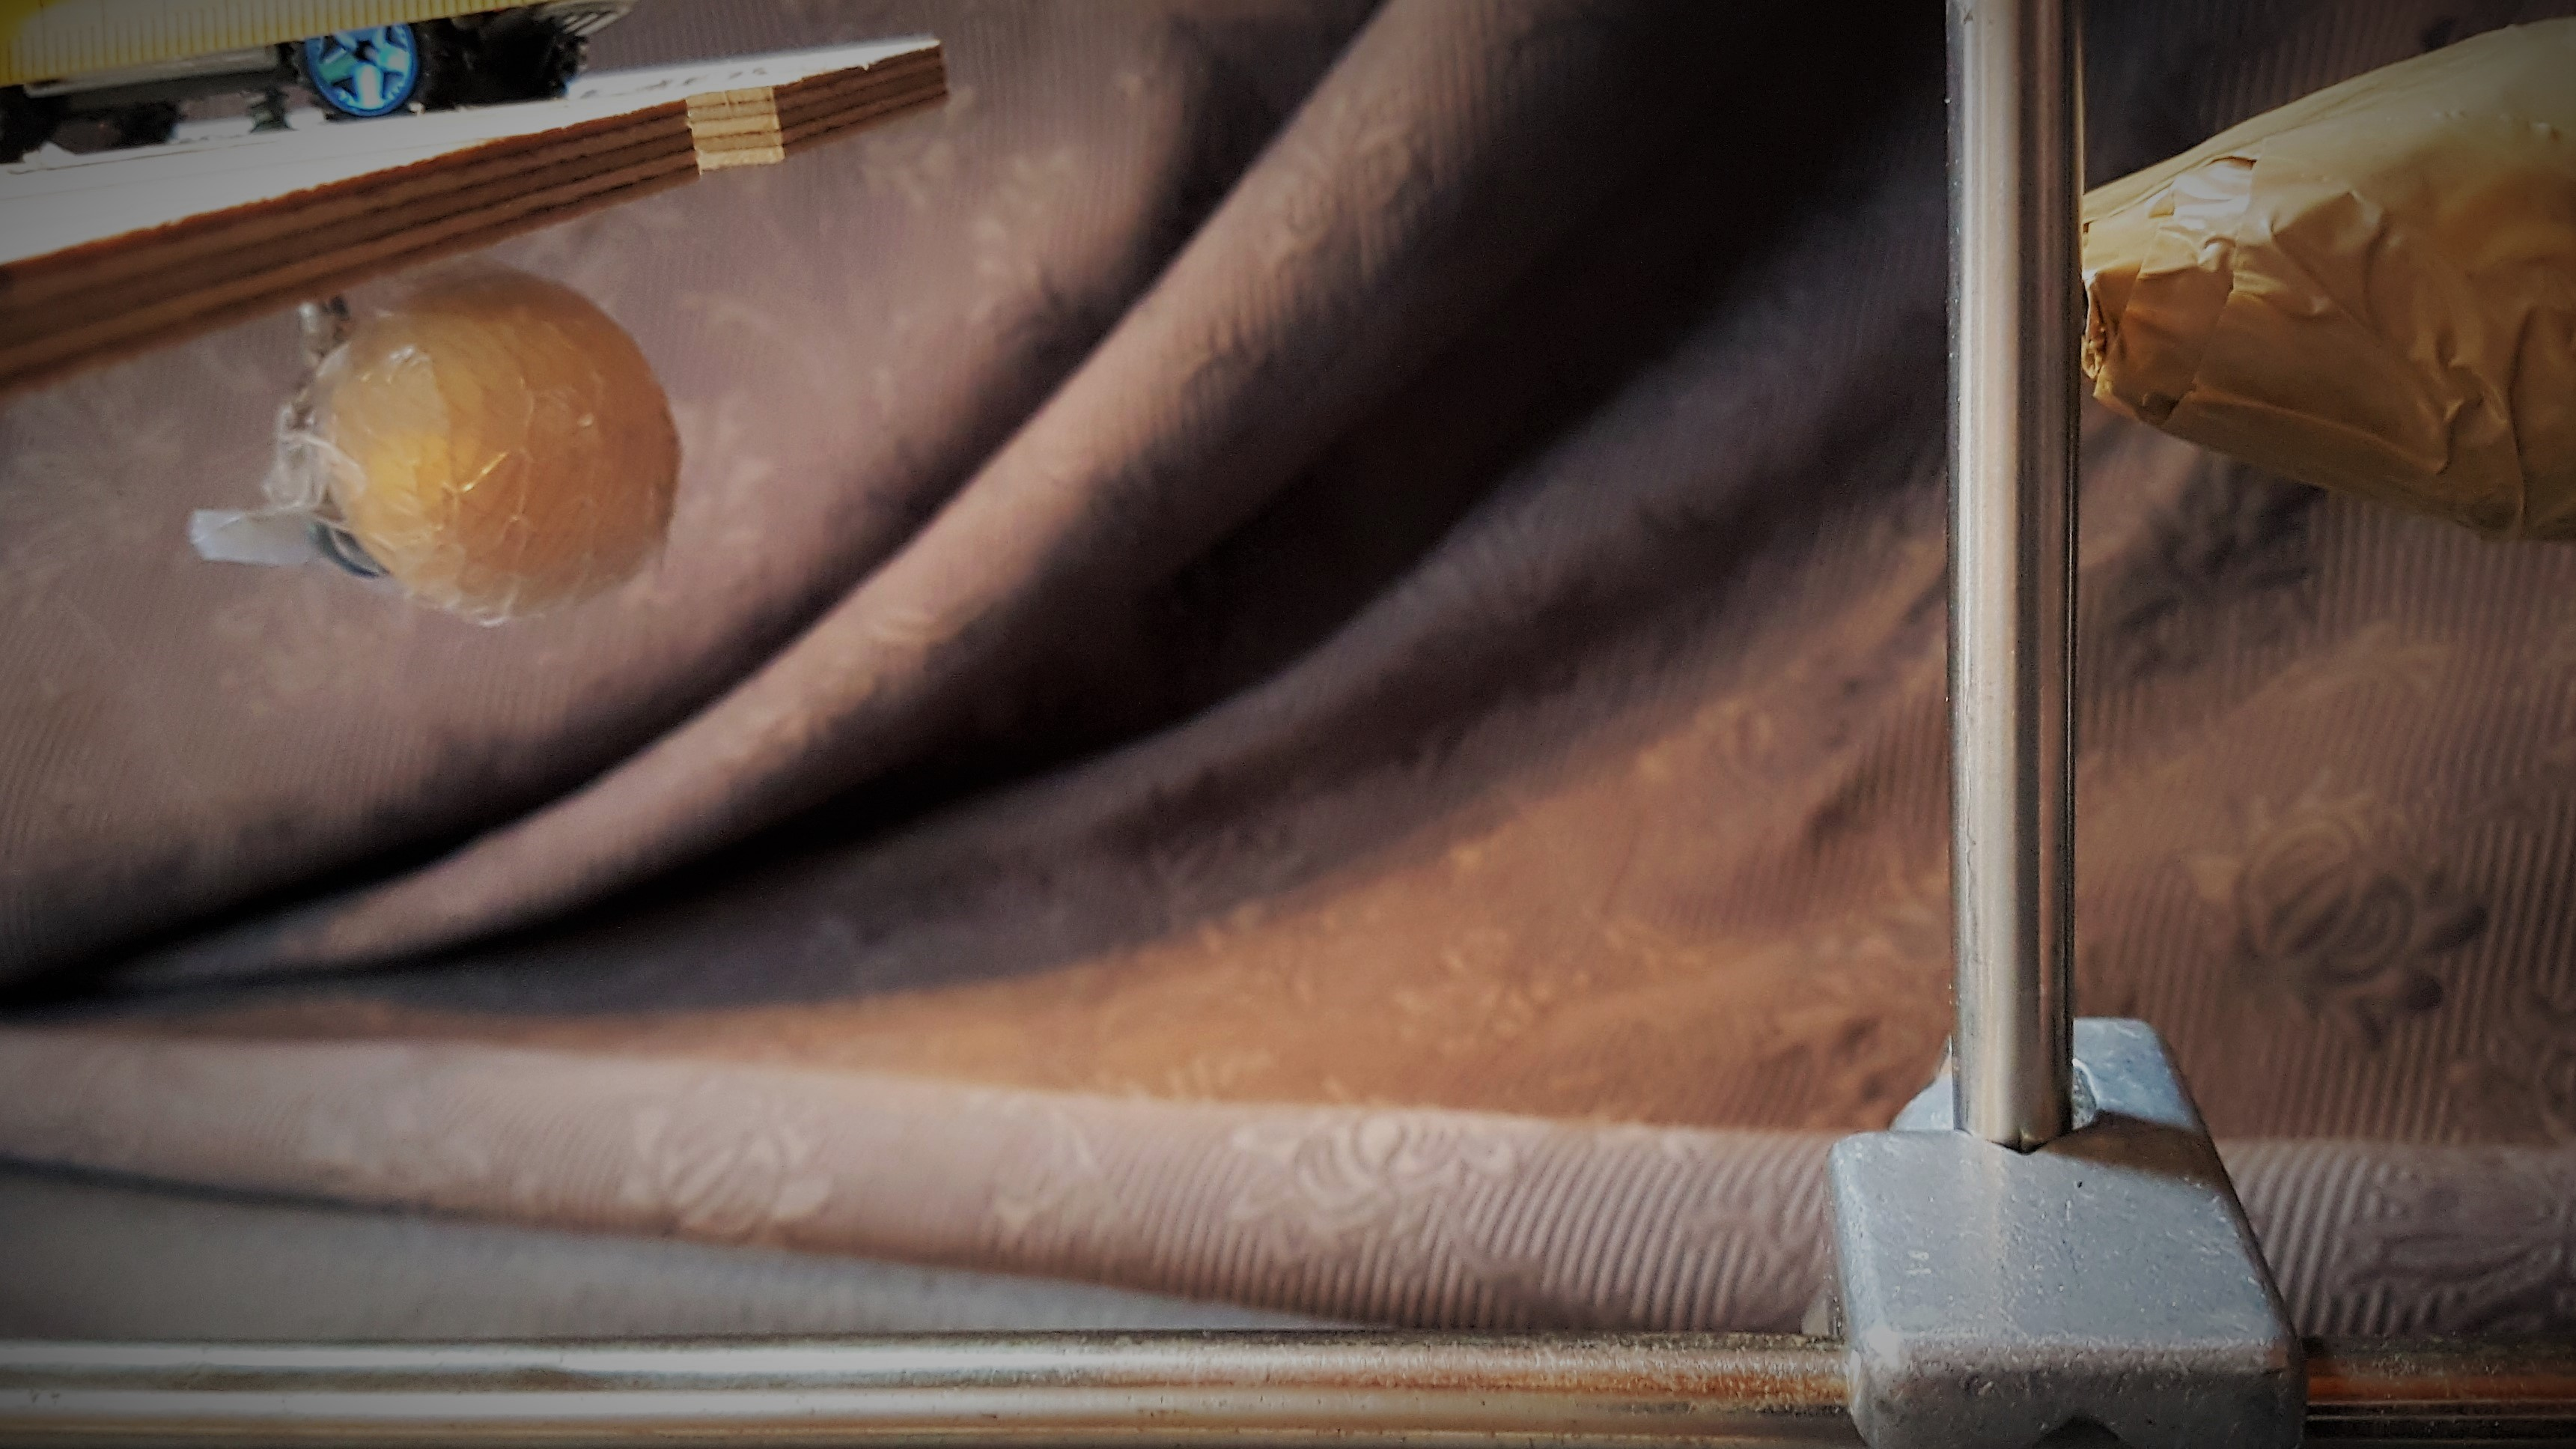
\includegraphics[scale=0.027]{images/stroemungskraftmessung2.jpg}};  
\end{tikzpicture}
  \caption[Erster Versuchsaufbau zur Strömungskraftmessung]{Erster Versuchsaufbau zur Strömungskraftmessung: Ein Messwagen, an dem eine Kugel aufgehängt wird, ist mit einem Federkraftmesser über eine Umlenkrolle verbunden. Die Unterseite der Messplatte ist als Auszug links oben im Foto abgebildet.}
  \label{fig:stroemungskraftmessung1}
  \vspace{-0pt}
\end{figure}

\noindent Hierzu erhält ein Spielzeugauto eine Bohrung durch die Bodenplatte, um mit einem Haken den zu vermessenden Gegenstand anzubringen, und --- für die Verbindung mit dem Kraftmesser --- eine Bohrung am Heck. Als Messfläche wird eine dünne Sperrholzplatte genutzt, in welche eine schmale Aussparung für den unteren Haken gesägt wird. Um die Kraftmessung nur in eine Raumrichtung zuzulassen, werden mit einem Stechbeitel Schienen für den Messwagen in die Platte gehauen. Ein Foto des Versuchsaufbaus ist in Darstellung \ref{fig:stroemungskraftmessung1} abgebildet.

Bereits nach den ersten Messungen stellt sich allerdings heraus, dass der Versuchsaufbau aus mehreren Gründen ungeeignet ist
\begin{items}
\item Federkraftmesser haben einen relativ langen \textit{Hubweg}. Dadurch wird nur für einen Sekundenbruchteil der wahre Abstand des Föhns zu der Kugel vermessen, da der Messwagen einige Zentimeter vorwärts rollt, was in einem Ausschlag des Federkraftmessers auf eine Kraft $N_\mathrm{max}$ gesehen werden kann, deren Anzeigedauer jedoch nicht lang genug für eine Aufzeichnung ist.
\item Bei der Versuchsanordnung befindet sich der Ball nicht unmittelbar unterhalb der Platte, sondern in einem Abstand von ca. $\SI{1}{\centi\metre}$, was für eine Modellierung des Strömungsverhaltens im zu erstellenden Versuchsaufbau nicht hinnehmbar ist. Zudem ist das Sperrholzstück zu kurz, als dass das Gebläse direkt an ihm montiert werden könnte. Für verschiedene Messabstände ist jeweils eine zeitaufwendige Neukalibrierung erforderlich. 
\item Eine Messreihe von ausreichender Größe für eine mathematische Beschreibung benötigt sehr viele Messwerte, die nach \textcite{Schilling1987} im Bereich um $\SI{100}{\milli\newton}$ zu erwarten sind. Ein Federkraftmesser dieser Genauigkeit kann zwar beschafft werden, jedoch erfordern die näheren Föhnabstände $s$ bei größerem Kugelradius $r$ einen weiteren Kraftmesser für einen höheren Messbereich, was eine Vergleichbarkeit der Messungen wiederum unmöglich macht.
\end{items}

%% Autor: Björn Ritterbecks 
%% Letzte Aenderung: 15.06.2016 
\thisfloatsetup{%
  capbesidewidth=\marginparwidth}
\begin{figure}[htbp]
\centering
%\sansmath
 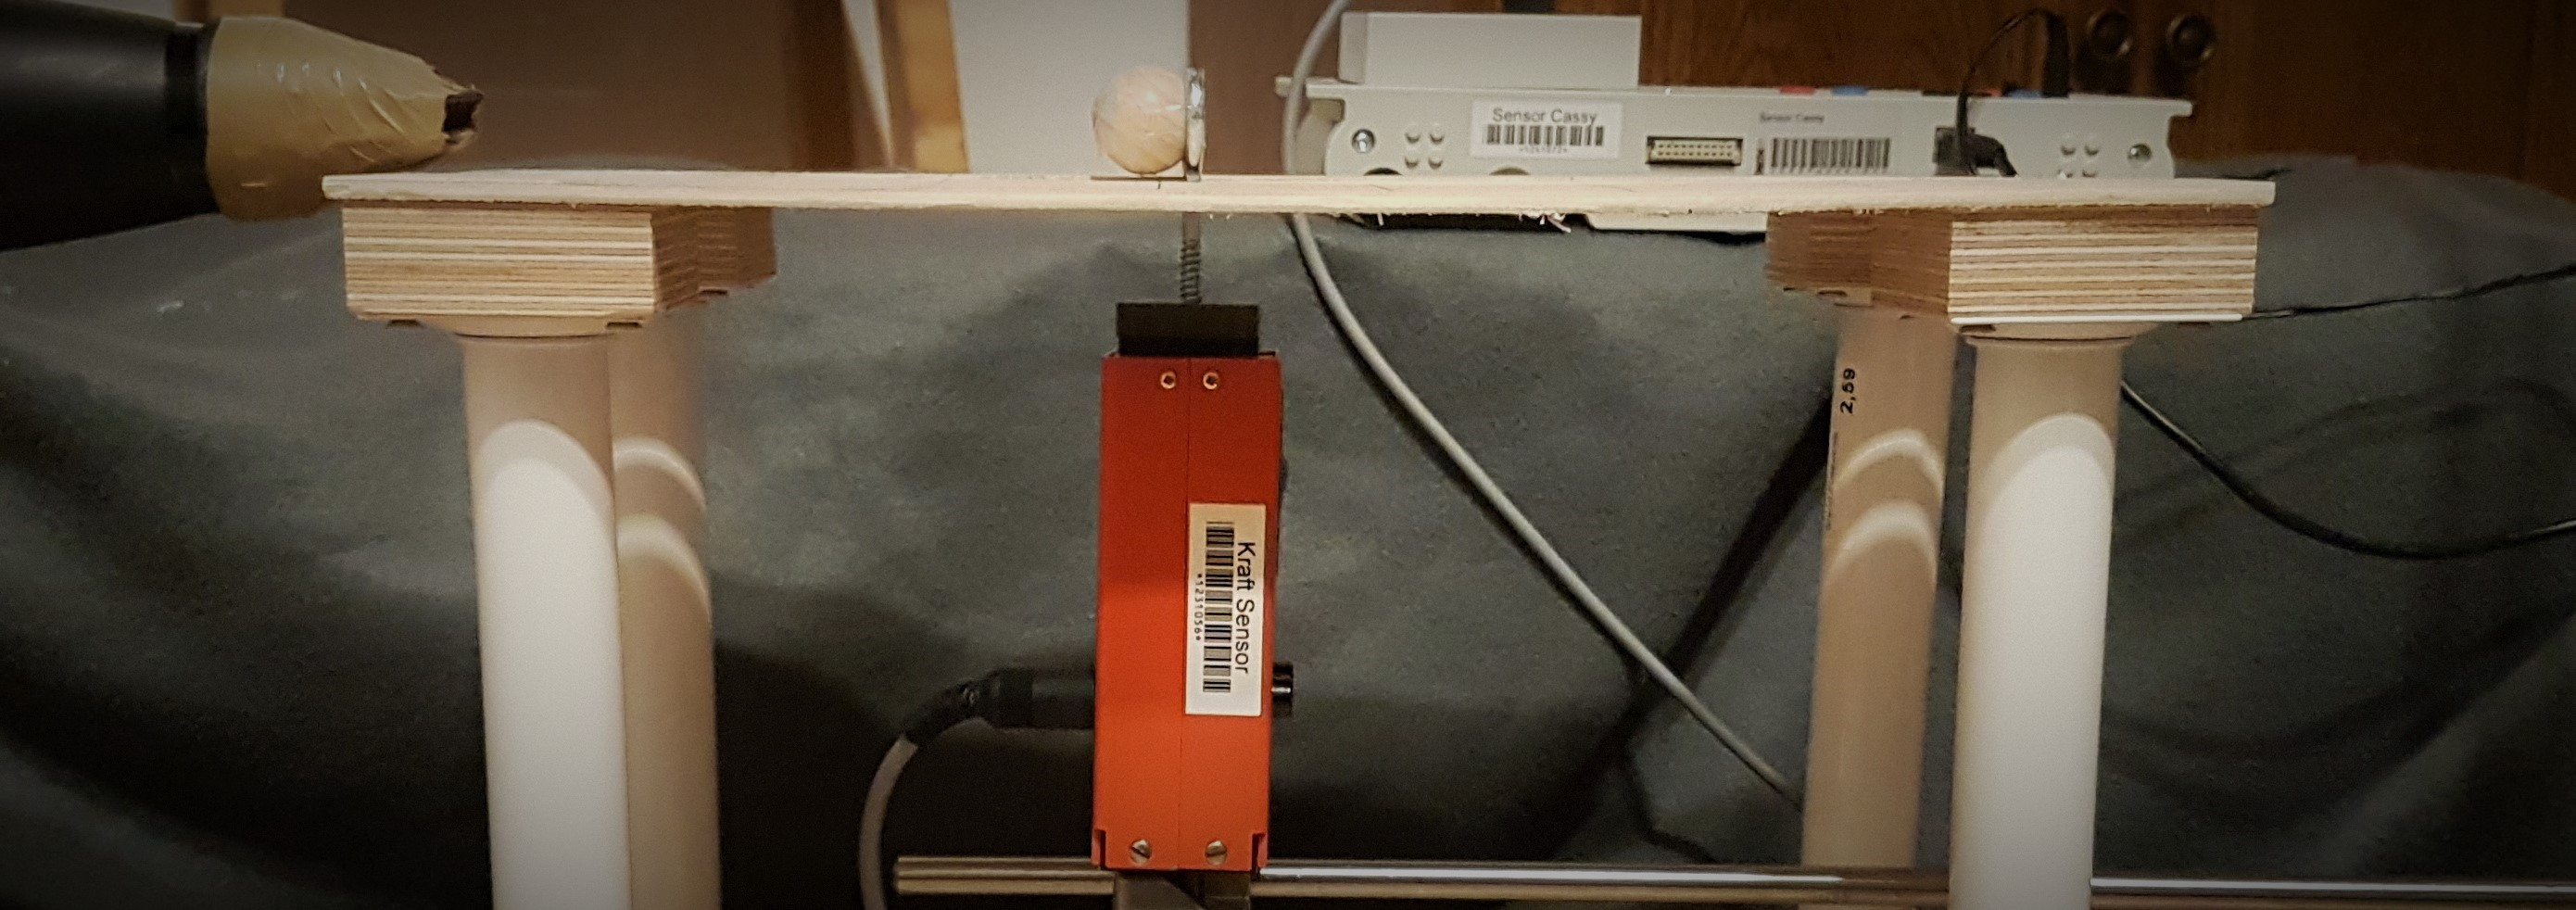
\includegraphics[width=0.99\textwidth]{images/stroemungskraftmessung3.jpg}
  \caption[Coulomb-Kraftmesser der Firma LD Didactic]{Die orange-farbige Box in der Mitte des Fotos vom Messaufbau ist ein Coulomb-Kraftmesser. Dieser ist in $x$-Richtung beweglich an eine Stativstange montiert. Ein eingeschraubter Haken ermöglicht die Befestigung von zu vermessenden Luftwiderständen.}
    \label{fig:stroemungskraftmessung3}
  \vspace{-0pt}
\end{figure}

\noindent Aus einem Schülerversuch sind \textit{Coulomb-Kraftmesser} bekannt (siehe Abbildung \ref{fig:stroemungskraftmessung3}), die auf ein hundertstel $\si{\milli\newton}$ genau messen können und zudem --- laut Herstellerangaben von \textsc{Leybold Didactic}\footnote{vgl. \url{http://www.ld-didactic.de/documents/de-DE/GA/GA/5/524/524060d.pdf}, abgerufen am 29.06.2016} --- einen Hub von lediglich $\pm \SI{0.5}{\milli\metre}$ haben, womit diese Kraftmesser alle zuvor genannten Bedingungen erfüllt. Von Vorteil ist auch, dass durch die Messwerterfassung mit \textsc{Cassy} über ein Zeitintervall gemittelte Werte und damit genauere Ergebnisse möglich sind.

%% Autor: Björn Ritterbecks 
%% Letzte Aenderung: 15.06.2016 
\thisfloatsetup{%
  capbesidewidth=\marginparwidth}
\begin{figure}[htbp]
\centering
%\sansmath
 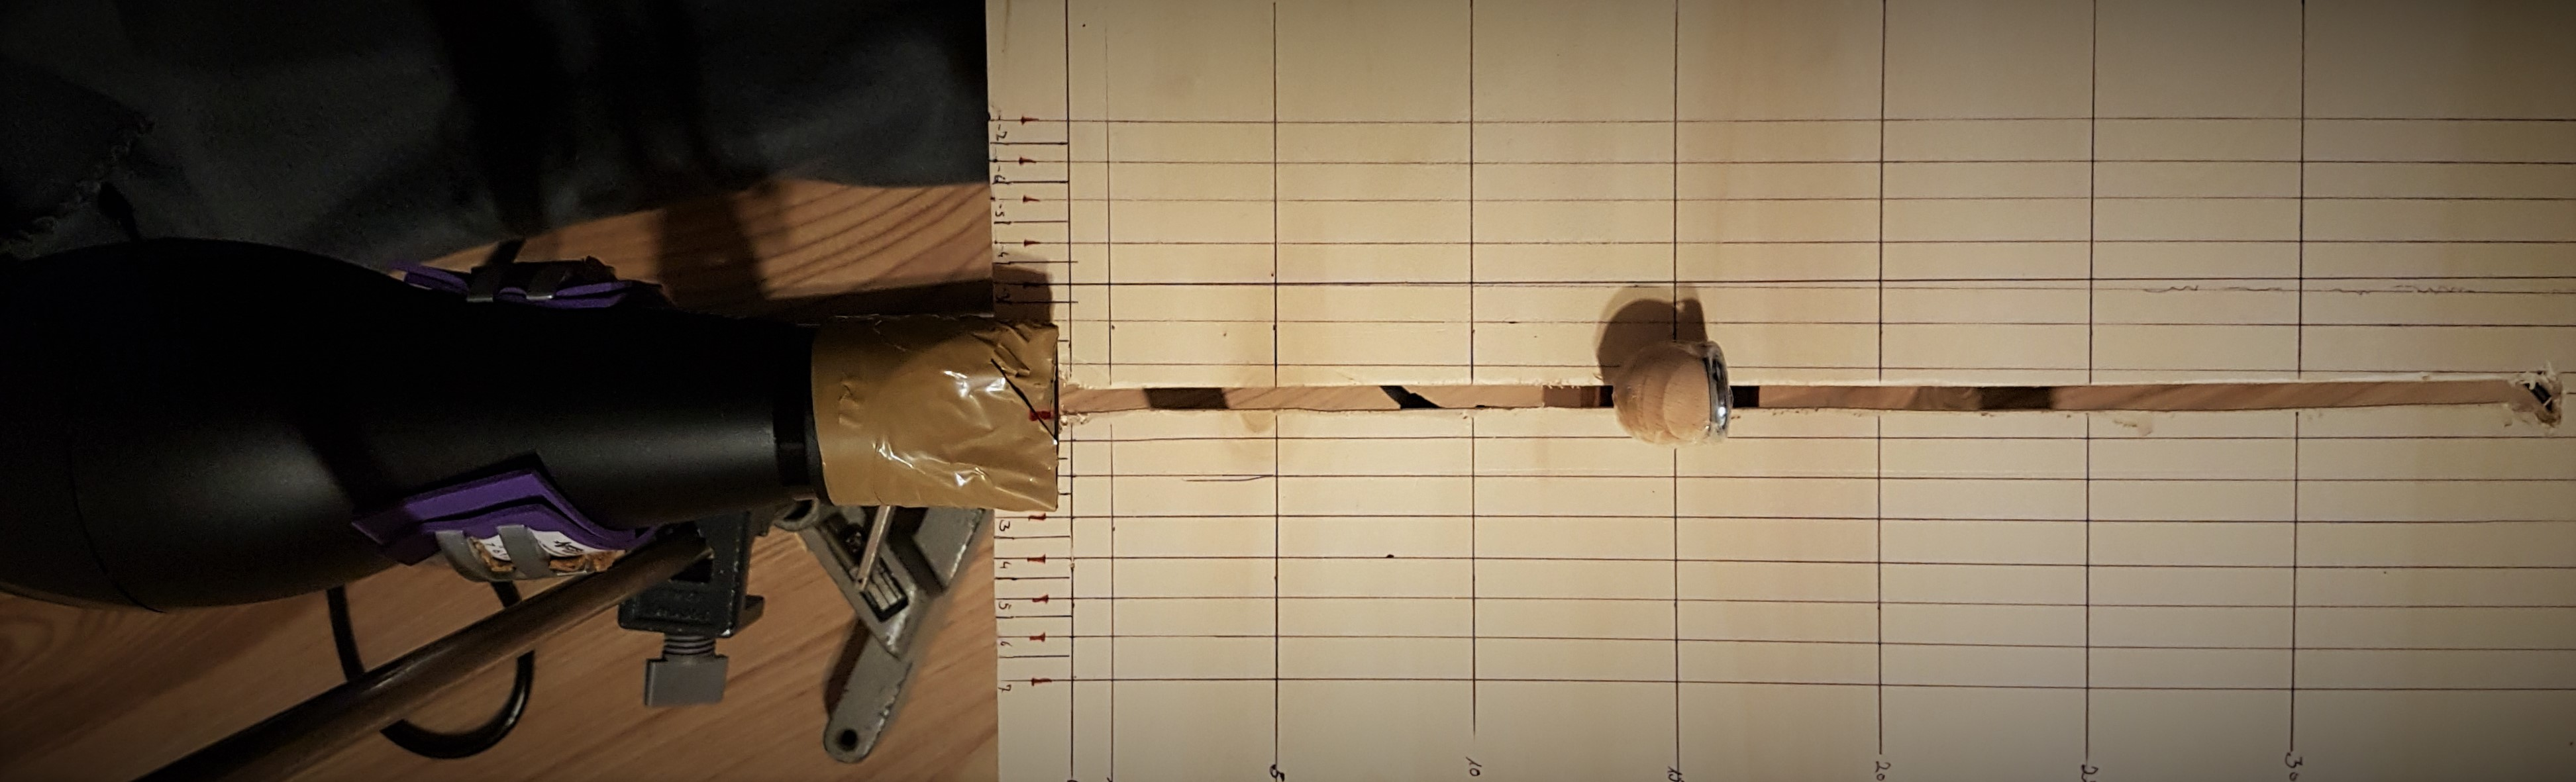
\includegraphics[width=0.99\textwidth]{images/stroemungskraftmessung4.jpg}
  \caption[Zweiter Versuchsaufbau zur Srömungskraftmessung]{Draufsicht des zweiten Versuchsaufbaus für die Messungen zur Strömungswiderstandskraft von Kugeln unterschiedlicher Radien. Ein Föhn ist beweglich auf einem Stativfuß an dem Messtisch angebracht, der mit einem Koordinatensystem für die Messreihen präpariert ist.}
  \label{fig:stroemungskraftmessung4}
  \vspace{-0pt}
\end{figure}

\noindent Ein Messtisch der Länge $l=\SI{35}{\centi\metre}$, der aus Sperrholz und Möbelfüßen schnell hergestellt ist, erhält ein Koordinatensystem, um die Datenerfassung zuverlässig und zügig vornehmen zu können. In die Bohrung des Coulomb-Kraftmessers wird von oben durch eine Ausfräsung des Messtisches ein mit einer Kugel beklebter Haken geschraubt. Durch diesen Aufbau ist es möglich, die Bälle direkt oberhalb der Platte, jedoch reibungsfrei zu lagern. Das Gebläse, wird auf einem schweren Stativ so angebracht, dass die Düsenöffnung $\SI{2}{\centi\metre}$ in die Platte hineinragt.

Die 56 Messreihen (4 Kugelradien á 7 Abstände á 2 Gebläsestufen) werden folgendermaßen aufgezeichnet: Der Kraftmesser wird in einem festen Abstand $s_i$ zum Föhn fixiert. Dieser wird anschließend möglichst parallel zur $x$-Achse auf die $\SI{5}{\milli\metre}$ auseinanderliegenden Messpunkte geführt, wo nach einer Integrationszeit von $\SI{300}{\milli\second}$ der jeweilige Messwert von der Benutzeroberfläche des \textit{Cassy-Lab 2} abgelesen wird. Die ersten beiden Messungen sind in Tabelle \ref{tab:kraftmessung1} aufgelistet.

  \thisfloatsetup{
  capbesidewidth=\marginparwidth,
}
\begin{table}[htb]
\centering
%\sffamily,
\small
%\sansmath
\arrayrulecolor{white}
%\setlength{\arrayrulewidth}{2pt}
\vspace{0.2cm}
  \rowcolors{2}{halfgray!15}{halfgray!5}
 \setlength{\extrarowheight}{.00em}
 \subfloat[$s=\SI{1}{\centi\metre}$]{
			\begin{tabularx}{0.45\textwidth}{r*{2}{>{\RaggedLeft\arraybackslash}X}}	
\rowcolor{mycolor} & 	\multicolumn{2}{c}{{\color{white}\textbf{Kraft in $\boldsymbol{\si{\milli\newton}}$}}} \\
\rowcolor{mycolor}  \multirow{-2}{*}{{\color{white}\textbf{$\boldsymbol{d}$ in $\boldsymbol{\si{\centi\metre}}$}}} & \multicolumn{1}{c}{{\color{white}\textbf{Stufe 2}}} &\multicolumn{1}{c}{{\color{white}\textbf{Stufe 1}}}\\
-4,0	$\pm$	0,1	&	0	&	0	\\
-3,5	$\pm$	0,1	&	6	&	2	\\
-3,0	$\pm$	0,1	&	60	&	42	\\
-2,5	$\pm$	0,1	&	115	&	70	\\
-2,0	$\pm$	0,1	&	150	&	90	\\
-1,5	$\pm$	0,1	&	210	&	122	\\
-1,0	$\pm$	0,1	&	276	&	177	\\
-0,5	$\pm$	0,1	&	303	&	188	\\
0,0	$\pm$	0,1	&	292	&	183	\\
0,5	$\pm$	0,1	&	263	&	165	\\
1,0	$\pm$	0,1	&	214	&	128	\\
1,5	$\pm$	0,1	&	154	&	97	\\
2,0	$\pm$	0,1	&	114	&	68	\\
2,5	$\pm$	0,1	&	75	&	52	\\
3,0	$\pm$	0,1	&	23	&	14	\\
3,5	$\pm$	0,1	&	0	&	0	\\
		\end{tabularx}}
		\quad
 \subfloat[$s=\SI{5}{\centi\metre}$]{
			\begin{tabularx}{0.45\textwidth}{r*{2}{>{\RaggedLeft\arraybackslash}X}}	
\rowcolor{mycolor} & 	\multicolumn{2}{c}{{\color{white}\textbf{Kraft in $\boldsymbol{\si{\milli\newton}}$}}} \\
\rowcolor{mycolor}  \multirow{-2}{*}{{\color{white}\textbf{$\boldsymbol{d}$ in $\boldsymbol{\si{\centi\metre}}$}}} & \multicolumn{1}{c}{{\color{white}\textbf{Stufe 2}}} &\multicolumn{1}{c}{{\color{white}\textbf{Stufe 1}}}\\
-4,0	$\pm$	0,2	&	0	&	0	\\
-3,5	$\pm$	0,2	&	3	&	0	\\
-3,0	$\pm$	0,2	&	32	&	5	\\
-2,5	$\pm$	0,2	&	67	&	35	\\
-2,0	$\pm$	0,2	&	111	&	71	\\
-1,5	$\pm$	0,2	&	170	&	104	\\
-1,0	$\pm$	0,2	&	217	&	145	\\
-0,5	$\pm$	0,2	&	249	&	156	\\
0,0	$\pm$	0,2	&	250	&	157	\\
0,5	$\pm$	0,2	&	235	&	146	\\
1,0	$\pm$	0,2	&	205	&	121	\\
1,5	$\pm$	0,2	&	159	&	84	\\
2,0	$\pm$	0,2	&	114	&	62	\\
2,5	$\pm$	0,2	&	65	&	30	\\
3,0	$\pm$	0,2	&	10	&	2	\\
3,5	$\pm$	0,2	&	0	&	0	\\
		\end{tabularx}}		
		\caption[Exemplarische Kraftmessung des Gebläses]{Exemplarische Kraftmessung des Gebläses für eine Kugel mit $r=\SI{17.5}{\milli\metre}$ bei einem Abstand von \textbf{\color{mycolor}(a)}, $s=\SI{1}{\centi\metre}$ und \textbf{\color{mycolor}(b)}, $s=\SI{5}{\centi\metre}$ vom Föhn, der über zwei Gebläsestufen verfügt. Die Aufnahme der Messdaten erfolgt mit einem \textsw{Coulomb-Kraftmesser}.} 
		\label{tab:kraftmessung1}	
		\end{table} %\vspace*{-5cm}\newpage

\noindent Die Messungenauigkeit auf die Kraft $F_\mathrm{LW}$ beträgt nach den Herstellerangaben des verwendeten Gerätes $\SI{1}{\percent}$, womit sie gegenüber der Justage des Gebläses vernachlässigbar ist. Wird der Haartrockner nicht genau parallel zur $x$-Achse ausgerichtet, so ergibt sich über den Tangens bei zunehmendem Abstand $s$ eine Entfernungsdifferenz $\Delta s$ von bis zu $\SI{1.1}{\centi\metre}$, wenn davon ausgegangen wird, dass die Ausrichtung nur auf $\SI{2}{\degree}$ genau erfolgt (hierzu sei auf grafische Auftragungen wie \ref{fig:kraftmessung9} im Anhang verwiesen, bei denen eine \textit{Schiefe} erkannt werden kann). Selbst bei der als gering angenommenen Abweichung übertrifft diese Unsicherheit diejenige des Messgerätes um den Faktor fünf.

  \thisfloatsetup{%
  capbesidewidth=\marginparwidth}

\begin{figure}[htbp]
\centering
%\sansmath
\subfloat[Stufe 2]{
\begin{tikzpicture}
\begin{axis}[	
	clip=false, % Verhindet weiße Punkte bei vielfach geplotteten x-Werten
	ymajorgrids,
    xmajorgrids,
          axis x line*=middle,
          axis y line*=center,
    grid style={white},
	axis on top,
    width=12cm,
    height=4.797cm,
    xmin=-7,
    xmax=7,
    ymin=0,
    ymax=350,
    %/tikz/ybar interval,
    tick align=center,
    xtick align=outside,
    xlabel={Abstand $d$},
    ylabel={\rotatebox[origin=b]{270}{Windlast $F_\mathrm{LW}$}},   
   x label style={at={(axis cs:5,-65)}},
    y label style={at={(axis cs:-3.5,300)}},
    axis line style={Honeydew4!70!black},
    ticklabel style={Honeydew4!70!black, inner sep=1pt,
                font=\footnotesize},
    yticklabels={${50}$, ${100}$, ${150}$,  ${200}$,   ${250}$ , ${\si{\milli\newton}}$, ${350}$ },            
    ytick={50,100,150,200, 250, 300, 350},
    xticklabels={-7,-5,-3,-1,1,3, $\si{\centi\metre}$, 7},
     xtick={-7,-5,-3,-1,1,3,5, 7}, 
    scaled ticks=false,
    width=\textwidth,                                   
    label style={font=\small,Honeydew4!70!black,},
    enlarge x limits=true,
    %tick style={draw=none},
    x tick label as interval=false,
]
\draw[thick, Honeydew4!70!black, ->,>={latex[Honeydew4!70!black, round, length=0.4cm, width=4pt]}] (axis cs:-3.50, 260) -- (axis cs:-3.50, 340);
\draw[thick,Honeydew4!70!black, ->,>={latex[Honeydew4!70!black,round, length=0.4cm, width=4pt]}] (axis cs:3.00, -65) -- (axis cs:7.00, -65);
\addplot[fill=mycolor4, draw=mycolor4, only marks, mark=*, error bars/.cd,
   x dir=both,
   x explicit, error bar style={mycolor4}]
table[x = x, y =y, x error=dx]{images/data/kraftmessung1S2.dat};
\addplot[mycolor, fill=mycolor!25, smooth, domain=-8:8,thick, opacity=0.4] {302.8*exp(-((x)/2.143)^2)};
\end{axis}
\clipright
\end{tikzpicture}}
\\
\subfloat[Stufe 1]{
\begin{tikzpicture}
\begin{axis}[	
	clip=false, % Verhindet weiße Punkte bei vielfach geplotteten x-Werten
	ymajorgrids,
    xmajorgrids,
          axis x line*=middle,
          axis y line*=center,
    grid style={white},
	axis on top,
    width=12cm,
    height=4.797cm,
    xmin=-7,
    xmax=7,
    ymin=0,
    ymax=350,
    %/tikz/ybar interval,
    tick align=center,
    xtick align=outside,
    xlabel={Abstand $d$},
    ylabel={\rotatebox[origin=b]{270}{Windlast $F_\mathrm{LW}$}},   
   x label style={at={(axis cs:5,-65)}},
    y label style={at={(axis cs:-3.5,300)}},
    axis line style={Honeydew4!70!black},
    ticklabel style={Honeydew4!70!black, inner sep=1pt,
                font=\footnotesize},
    yticklabels={${50}$, ${100}$, ${150}$,  ${200}$,   ${250}$ , ${\si{\milli\newton}}$, ${350}$ },            
    ytick={50,100,150,200, 250, 300, 350},
    xticklabels={-7,-5,-3,-1,1,3, $\si{\centi\metre}$, 7},
     xtick={-7,-5,-3,-1,1,3,5, 7}, 
    scaled ticks=false,
    width=\textwidth,                                   
    label style={font=\small,Honeydew4!70!black,},
    enlarge x limits=true,
    %tick style={draw=none},
    x tick label as interval=false,
]
\draw[thick, Honeydew4!70!black, ->,>={latex[Honeydew4!70!black, round, length=0.4cm, width=4pt]}] (axis cs:-3.50, 260) -- (axis cs:-3.50, 340);
\draw[thick,Honeydew4!70!black, ->,>={latex[Honeydew4!70!black,round, length=0.4cm, width=4pt]}] (axis cs:3.00, -65) -- (axis cs:7.00, -65);
\addplot[fill=mycolor, draw=mycolor, only marks, mark=*, error bars/.cd,
   x dir=both,
   x explicit, error bar style={mycolor}]
table[x = x, y =y, x error=dx]{images/data/kraftmessung1S1.dat};
\addplot[mycolor4, fill=mycolor4!25, smooth, domain=-8:8,thick, opacity=0.4] {188.1*exp(-((x)/2.133)^2)};
\end{axis}
\clipright
\end{tikzpicture}}
  \caption[Beispielhafter Gaußglocken-Fit]{Beispiel eines in \textit{Matlab} erzeugten Gaußglocken-Fits für die Messung der Kugel mit $r=\SI{17.5}{\milli\metre}$ bei einem Abstand von $s=(1.0\pm 0.1)\,\si{\centi\metre}$. Als Anpassungsfunktion wird für alle Messreihen $f(d)=A\cdot \exp(-\left(\sfrac{d-\mu}{2\sigma^2}\right)^2)$ verwendet, da sie im Mittel die geringsten quadratischen Abweichungen bei den vorhandenen Daten liefert. Alle graphischen Auftragungen der Messwerte wurden um das jeweilige $\mu$ verschoben. Die Fehlerbalken sind kaum zu erkennen, da als Unsicherheit auf den Abstand des Gebläses von der Mittelachse ein Winkel von $\varphi=\SI{2}{\degree}$ angenommen wird und damit die Messungenauigkeit linear mit dem Abstand des Föhns skaliert. }
  \label{fig:kraftmessung1}
  \vspace{-0pt}
\end{figure}

\noindent Abbildung \ref{fig:kraftmessung1} zeigt die Diagramme zu den Messwerten aus Tabelle \ref{tab:kraftmessung1}. Die Kurvenanpassung in Form einer Gaussglocke, die mit der Software \textit{Matlab} berechnet wird, folgt dem Modell
\begin{equation}
\label{eq:gebl1}
f(d)=A\cdot \e^{-\left(\frac{d-\mu}{2\sigma^2}\right)^2},
\end{equation}
welches eine klassische \textit{Gaußverteilung} darstellt (siehe Tab. \ref{tab:gaaussfit1}). Werden nun die Integrale unterhalb der Kurven berechnet, so können diese als \textit{an den Kugeln verrichtete Arbeit} $W$ gesehen werden, wobei die Lösung durch die Verschiebung der Messpunkte um $\mu$ das Integral vereinfacht:
\begin{equation}
\label{eq:gebl2}
\begin{alignedat}{2}
 W & = \int_{d_\mathrm{min}}^{d_\mathrm{max}}A\cdot \e^{-\frac{d}{2\sigma^2}^2}\mathrm{d}d\\
 & = \frac{1}{2}\sqrt{\uppi}\cdot A\cdot 2\sigma^2 \cdot \mathrm{erf}(\frac{d}{2\sigma^2}),
\end{alignedat}
\end{equation}
wobei $\mathrm{erf}(\sfrac{d}{2\sigma^2})$ die \textit{gauß'sche Fehlerfunktion}
\begin{equation}
\mathrm{erf}(\frac{d}{2\sigma^2})=\frac{2}{\sqrt{\uppi}}\int_{0}^{\sfrac{d}{2\sigma^2}}\e^{-\tau^2}\mathrm{d}\tau
\end{equation}
bezeichnet. Die Funktion ist punktsymmetrisch zum Koordinatenursprung und konvergiert bereits ab $x=\pm 1$ schnell gegen $\pm 1$. Wie \textsc{Bronstein} aufführt, gilt zudem 
\begin{equation}
2\Phi (x)-1=\mathrm{erf}(\frac{x}{\sqrt{\uppi}}),
\end{equation} 
die Fehlerfunktion kann demnach mit der \textit{Standardnormalverteilung} $\Phi(x)$ berechnet werden.\footfullcite[vgl.][S.\,517]{Bronstein2008}

  \thisfloatsetup{
  capbesidewidth=\marginparwidth,
}
\begin{table}[htb]
\centering
%\sffamily,
\small
%\sansmath
\arrayrulecolor{white}
%\setlength{\arrayrulewidth}{2pt}
\vspace{0.2cm}
  \rowcolors{2}{halfgray!15}{halfgray!5}
 \setlength{\extrarowheight}{.00em}
			\begin{tabularx}{0.99\textwidth}{*{2}{>{\RaggedLeft\arraybackslash}X}X*{3}{>{\RaggedLeft\arraybackslash}X}}	
\rowcolor{mycolor}  {\color{white}\textbf{ Radius $\boldsymbol{r}$ in $\boldsymbol{\si{\milli\metre}}$}} & {\color{white}\textbf{Abstand $\boldsymbol{s}$ in $\boldsymbol{\si{\centi\metre}}$}} & {\color{white}\textbf{Amplitude $\boldsymbol{A}$ in $\boldsymbol{\si{\milli\newton}}$}} & {\color{white}\textbf{$\boldsymbol{\mu}$}} & {\color{white}\textbf{$\boldsymbol{2\sigma^2}$}}& {\color{white}\textbf{$\boldsymbol{R^2}$}}\\
	&	1	&	302,8	&	2,143	&	-0,240	&	0,994	\\
	&	5	&	260,4	&	2,099	&	-0,050	&	0,993	\\
	&	10	&	183,9	&	2,378	&	-0,378	&	0,993	\\
	&	15	&	152,8	&	2,349	&	-0,201	&	0,995	\\
	&	20	&	121,4	&	2,604	&	-0,404	&	0,997	\\
	&	25	&	95,2	&	3,650	&	-0,444	&	0,986	\\
\multirow{-7}{*}{17,5}	&	30	&	73,2	&	3,518	&	-0,626	&	0,992	\\\midrule
	&	1	&	230,9	&	1,903	&	-0,268	&	0,997	\\
	&	5	&	199,2	&	1,912	&	-0,489	&	0,988	\\
	&	10	&	140,9	&	2,201	&	-0,564	&	0,988	\\
	&	15	&	106,5	&	2,381	&	-0,452	&	0,997	\\
	&	20	&	85,2	&	2,609	&	-0,374	&	0,997	\\
	&	25	&	65,7	&	3,237	&	-0,746	&	0,996	\\
\multirow{-7}{*}{15,0}	&	30	&	55,9	&	3,755	&	-0,526	&	0,978	\\\midrule
	&	1	&	157,9	&	1,870	&	-0,484	&	0,994	\\
	&	5	&	139,7	&	1,923	&	-0,660	&	0,988	\\
	&	10	&	100,9	&	1,873	&	-0,596	&	0,994	\\
	&	15	&	73,3	&	2,219	&	-0,855	&	0,995	\\
	&	20	&	60,1	&	2,665	&	-0,345	&	0,994	\\
	&	25	&	44,9	&	2,868	&	-1,262	&	0,996	\\
\multirow{-7}{*}{12,5}	&	30	&	39,9	&	3,689	&	-1,572	&	0,992	\\\midrule
	&	1	&	104,1	&	1,733	&	-0,631	&	0,996	\\
	&	5	&	83,6	&	1,693	&	-0,501	&	0,988	\\
	&	10	&	66,7	&	1,799	&	-0,496	&	0,993	\\
	&	15	&	49,9	&	1,735	&	-0,492	&	0,990	\\
	&	20	&	38,9	&	2,302	&	-0,594	&	0,991	\\
	&	25	&	29,3	&	2,512	&	-0,780	&	0,976	\\
\multirow{-7}{*}{10,0}	&	30	&	25,2	&	2,768	&	-1,538	&	0,987	\\
		\end{tabularx}
		\caption[Ergebnisse der Gaußanpassungen für die höhere Gebläsestufe]{Ergebnisse der Gauß-Anpassungen für die Messreihen auf der höheren Gebläsestufe. $\mu$ und $\sigma$ sind ohne Einheit aufgeführt, da das Argument einer Exponentialfunktion stets dimensionslos ist. Wollte man sie mit aufführen, so wäre $[\mu]=\si{\metre}$ und $[\sigma] = \sqrt{\si{\metre}}$. Als Bestimmtheitsmaß wird $R^2$ gewählt, das für eine Anpassung, die keine \textsw{Residuen} übriglasst, den Wert eins annimmt.}
		\label{tab:gaaussfit1}	
		\end{table} %\vspace*{-5cm}\newpage

\noindent\textcite{Schilling1987} nehmen als verrichtete Arbeit das gesamte Integral unter $F_\mathrm{LW}(d)$ an. Sind die Kugeln jedoch weiter von dem Gebläse entfernt, sind sie aufgrund der Anordnung des Analogieexperiments mit seinen zwei disjunkten Platten diejenigen, welche zu den \textit{schnellen} (nur bis zu $\SI[fraction-function=\sfrac]{1}{\metre\per\second}$, womit das Adjektiv nicht überbewertet werden sollte) Kugeln gezählt werden, kürzer im Zentrum des Strömungsfeldes. 
Als Richtwert wird daher angenommen, dass sich die Kugeln bei einer Fixierung der Gebläse-Position bei $x=\SI{0}{\centi\metre}$ von $x=-\SI{3}{\centi\metre}$ bis $x=\SI{3}{\centi\metre}$ im Strömungsfeld befinden.

  \thisfloatsetup{%
  capbesidewidth=\marginparwidth
  }
\begin{figure}[htbp]
\centering
%\sansmath
\subfloat[]{
\begin{tikzpicture}
\begin{scope}[scale=0.98]
\begin{axis}[	
	clip=false, % Verhindet weiße Punkte bei vielfach geplotteten x-Werten
	ymajorgrids,
    xmajorgrids,
          axis x line*=middle,
          axis y line*=center,
    grid style={white},
	axis on top,
    width=\textwidth,  
    height=6.797cm,
    xmin=0,
    xmax=30,
    ymin=0,
    ymax=1200,
    %/tikz/ybar interval,
    tick align=center,
    xtick align=outside,
    xlabel={Entfernung $s$},
    ylabel={\rotatebox[origin=b]{270}{Arbeit $W$}},   
   x label style={at={(axis cs:25,-150)}},
    y label style={at={(axis cs:-3.0,780)}},
    axis line style={Honeydew4!70!black},
    ticklabel style={Honeydew4!70!black, inner sep=1pt,
                font=\footnotesize},
    yticklabels={${200}$, ${400}$, ${600}$,  ${800}$,  ${\si{\milli\newton\centi\metre}}$, ${1200}$ },            
    ytick={200,400,600, 800, 1000, 1200},
    xticklabels={0, 5, 10, 15, 20, $\si{\centi\metre}$, 30},
     xtick={0,5,10,15,20,25,30}, 
    scaled ticks=false,           
           legend style ={ at={(axis cs:30,1200)}, 
     anchor=north east, draw=none, 
         fill=none,align=left, text=Honeydew4!70!black,
          font=\footnotesize},               
    label style={font=\small,Honeydew4!70!black,},
    cycle list name=mycolor4 white,
    enlarge x limits=true,
    %tick style={draw=none},
    x tick label as interval=false,
]
\draw[thick, Honeydew4!70!black, ->,>={latex[Honeydew4!70!black, round, length=0.4cm, width=4pt]}] (axis cs:-5.50, 850) -- (axis cs:-5.50, 1150);
\draw[thick,Honeydew4!70!black, ->,>={latex[Honeydew4!70!black,round, length=0.4cm, width=4pt]}] (axis cs:21.00, -150) -- (axis cs:29.00, -150);
\addplot
table[x = x, y =y]{images/data/work1.dat};
\addlegendentry{$\SI{17.5}{\milli\metre}$};
\addplot
table[x = x, y =y]{images/data/work2.dat};
\addlegendentry{$\SI{15.0}{\milli\metre}$};
\addplot
table[x = x, y =y]{images/data/work3.dat};
\addlegendentry{$\SI{12.5}{\milli\metre}$};
\addplot
table[x = x, y =y]{images/data/work4.dat};
\addlegendentry{$\SI{10.0}{\milli\metre}$};
\end{axis}
\end{scope}
\clipright
\end{tikzpicture}}
\\
\subfloat[]{
\begin{tikzpicture}
\begin{scope}[scale=0.98]
\begin{axis}[	
	clip=false, % Verhindet weiße Punkte bei vielfach geplotteten x-Werten
	ymajorgrids,
    xmajorgrids,
          axis x line*=middle,
          axis y line*=center,
    grid style={white},
%	axis on top,
    width=\textwidth,  
    height=6.797cm,
    xmin=0,
    xmax=30,
    ymin=0,
    ymax=1200,
    %/tikz/ybar interval,
    tick align=center,
    xtick align=outside,
    xlabel={Entfernung $s$},
    ylabel={\rotatebox[origin=b]{270}{Arbeit $W$}},   
   x label style={at={(axis cs:25,-150)}},
    y label style={at={(axis cs:-3.0,780)}},
    axis line style={Honeydew4!70!black},
    ticklabel style={Honeydew4!70!black, inner sep=1pt,
                font=\footnotesize},
    yticklabels={${200}$, ${400}$, ${600}$,  ${800}$,  ${\si{\milli\newton\centi\metre}}$, ${1200}$ },            
    ytick={200,400,600, 800, 1000, 1200},
    xticklabels={0, 5, 10, 15, 20, $\si{\centi\metre}$, 30},
     xtick={0,5,10,15,20,25,30}, 
    scaled ticks=false,           
           legend style ={ at={(axis cs:30,1200)}, 
     anchor=north east, draw=none, 
         fill=none,align=left, text=Honeydew4!70!black,
          font=\footnotesize},               
    label style={font=\small,Honeydew4!70!black,},
    cycle list name=mycolor white,
    enlarge x limits=true,
    %tick style={draw=none},
    x tick label as interval=false,
]
\draw[thick, Honeydew4!70!black, ->,>={latex[Honeydew4!70!black, round, length=0.4cm, width=4pt]}] (axis cs:-5.50, 850) -- (axis cs:-5.50, 1150);
\draw[thick,Honeydew4!70!black, ->,>={latex[Honeydew4!70!black,round, length=0.4cm, width=4pt]}] (axis cs:21.00, -150) -- (axis cs:29.00, -150);
\addplot
table[x = x, y =y]{images/data/work1.dat};
\addlegendentry{$\SI{17.5}{\milli\metre}$};
\addplot
table[x = x, y =y]{images/data/work5.dat};
\addlegendentry{$\SI{15.0}{\milli\metre}$};
\addplot
table[x = x, y =y]{images/data/work6.dat};
\addlegendentry{$\SI{12.5}{\milli\metre}$};
\addplot
table[x = x, y =y]{images/data/work7.dat};
\addlegendentry{$\SI{10.0}{\milli\metre}$};
\addplot[mycolor, fill=none, smooth, domain=0:31,thick] {0.7145*\x^2-45.18*\x+1093};
\end{axis}
\end{scope}
\clipright
\end{tikzpicture}}
  \caption[An einer vorbeirollenden Kugel verrichtete Arbeit]{Geplottet sind die Arbeitsintegrale nach Gleichung \eqref{eq:gebl2}. {\color{mycolor}\textbf{(a)}:} Je kleiner der Kugelradius $r$, desto geringer ist die Strömungswiderstandskraft und damit auch das Integral über selbige. {\color{mycolor}\textbf{(a)}:} Durch Multiplikation der Arbeitsintegrale mit den Proportionalitätsfaktoren, welche aus den Kugelprojektionsflächen berechnet werden, kann die lineare Skalierung gezeigt werden.}
  \label{fig:workwork}
  \vspace{-0pt}
\end{figure}

\noindent Durch die Gleichung \eqref{eq:gebl2} werden die Arbeitsintegrale für die Sphären mit den Radien $r_1=\SI{10,0}{\milli\metre}$, $r_2=\SI{12,5}{\milli\metre}$, $r_3=\SI{15,0}{\milli\metre}$ und $r_4=\SI{17,5}{\milli\metre}$ berechnet. Mit Erinnerung an Abschnitt \ref{sec:umsetzung} wird von einer Proportionalität der Arbeit und damit auch der Impulsänderung mit der Projektionsfläche der Kugeln ausgegangen. Hierbei gilt $A_\mathrm{proj_1}\cdot 3,06=A_\mathrm{proj_2}\cdot 1,96=A_\mathrm{proj_3}\cdot 1,36=A_\mathrm{proj_4}$. Die Integrale sind in Abbildung \ref{fig:workwork} für die einzelnen Messreihen aufgetragen. Es ist gut zu sehen, dass die Hypothese angenommen werden kann, obwohl zwei Messreihen für die Kugel mit dem Radius $\SI{10}{\milli\metre}$ um bis zu $\SI{20}{\percent}$ unter den erwarteten Werten liegen. Für die eingezeichnete polynomische Anpassung wurde daher die kleinste Kugel nicht berücksichtigt.

\section{Geschwindigkeitsmessung der Anströmung}

Mit der ausgemessenen Kraftwirkung können ebenfalls die Widerstandsbeiwerte $c_\mathrm{W}$ berechnet und mit den Literaturwerten aus \ref{tab:cwwerte} verglichen werden, sofern die Geschwindigkeit der Anströmung bekannt ist.
Zu diesem Zweck wird ein simples \textit{Anemometer} \footnote{Windgeschwindigkeitsmesser} gebaut. Die Konstruktion kann an dem Foto \ref{fig:windgeschw1} erläutert werden:

%% Autor: Björn Ritterbecks 
%% Letzte Aenderung: 15.06.2016 
\thisfloatsetup{%
  capbesidewidth=\marginparwidth}
\begin{figure}[htbp]
\vspace*{0.2cm}
\centering
%\sansmath
 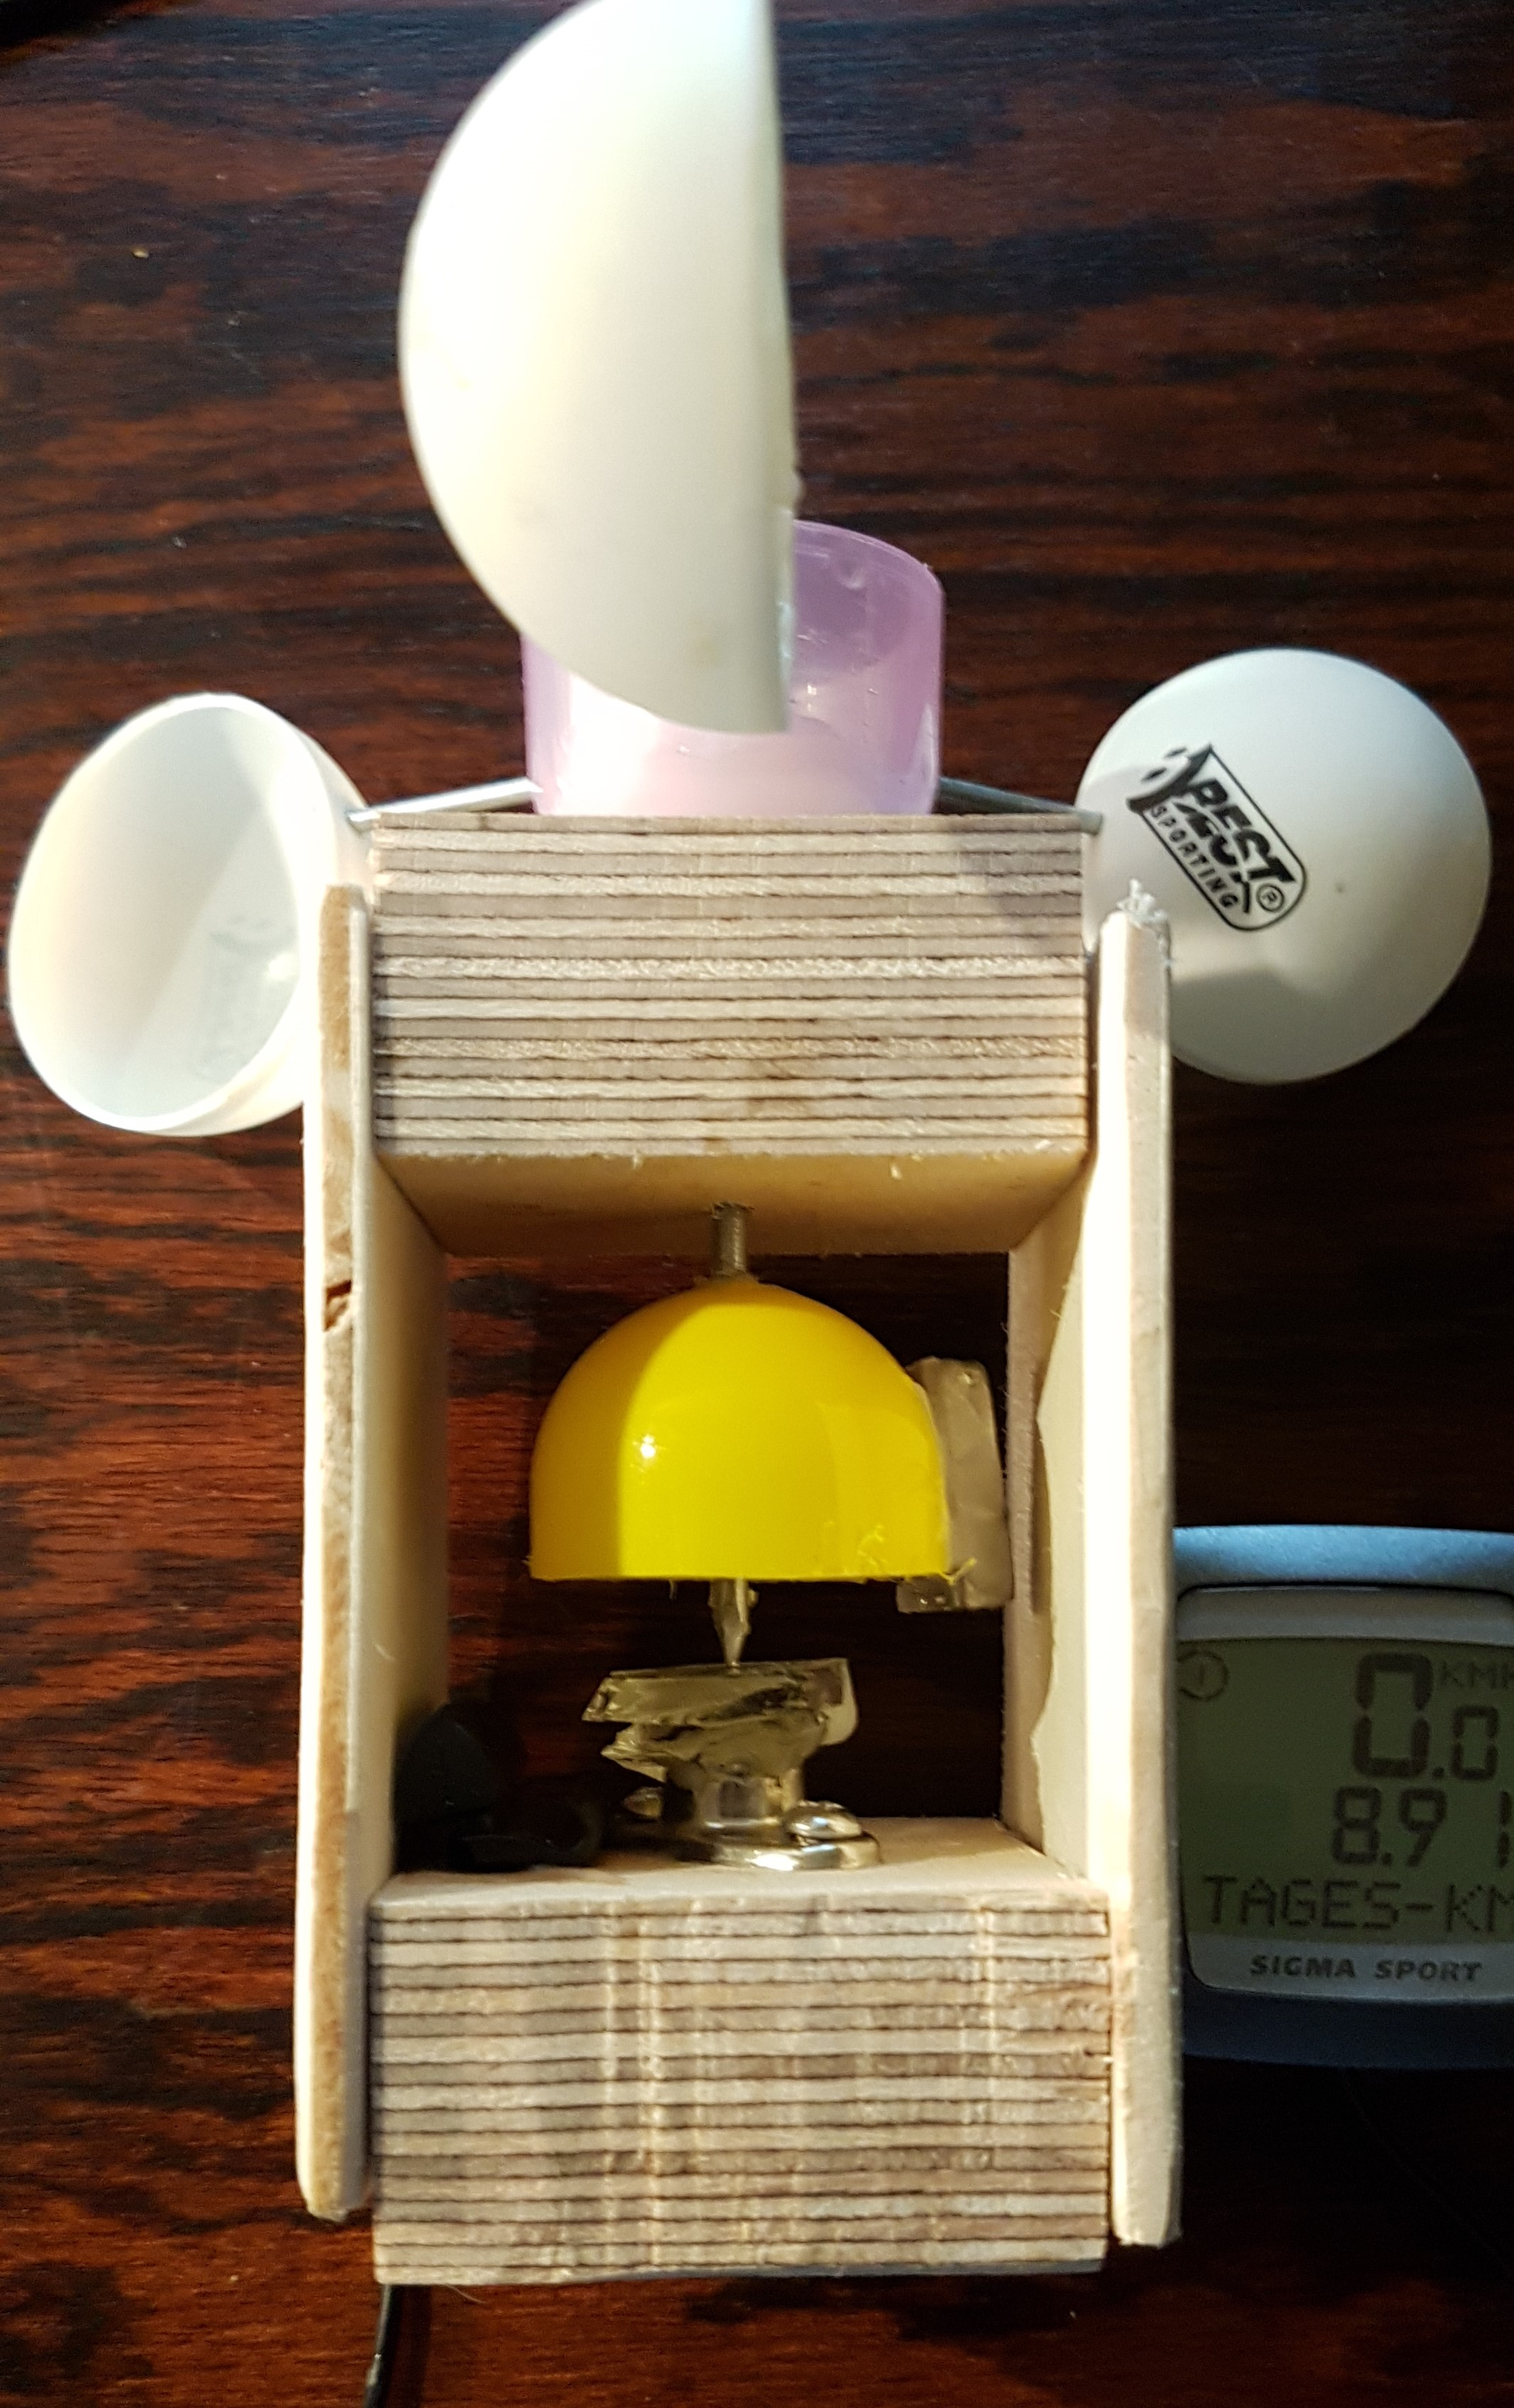
\includegraphics[width=0.75\textwidth]{images/Windkraft.jpg}
  \caption[Selbstbau eines Anemometers]{Aus einfachen Materialien und einem Fahrradcomputer gebautes Anemometer. Die Idee hinter dem Funktionsprinzip kommt von \textsc{Rüdiger Stenzel}: \url{http://www.dc4fs.de/wetter/anemo.htm}. Die Tischtennisballhälften drehen sich bei einem Luftstrom und versetzen damit einen Stahlstift in Rotation, an dem wiederum ein Magnet befestigt ist, der bei jeder Umdrehung durch einen \textsc{Reed-Kontakt} detektiert wird.}
  \label{fig:windgeschw1}
  \vspace{-0pt}
\end{figure}

\noindent Zwei Tischtennisbälle werden halbiert, um möglichst leichte Schalen zu erhalten. Am Rand jeder Hälfte wird ein kleines Loch gebohrt, durch welches ein Stahlnagel von $\SI{30}{\milli\metre}$ Länge gesteckt und anschließend eingeklebt wird. Drei dergestalt präparierte Schalen steckt man nun --- jeweils um $\SI{120}{\degree}$ gegeneinander verschränkt --- durch Bohrungen in der Verschlusskappe eines Kosmetikartikels oder ähnlichem. Hierbei fixieren die drei kurzen Stifte auch einen weiteren Nagel von mindestens $\SI{60}{\milli\metre}$ Länge, der orthogonal und mittig platziert wird, bevor die Kappe mit \textit{Epoxidharz} aufgefüllt wird.

Durch ein Stück dickeren Sperrholzes (in der Abbildung $\SI{30}{\milli\metre}$) wird ein Loch von $\SI{4}{\milli\metre}$ Durchmesser gebohrt, in welches ein passend abgelängter Teil eines Messingrohres mit gleichem Außendurchmesser eingeschlagen wird, um den langen Nagel möglichst \textit{lotrecht} durchzuführen. An dem unteren Ende des Stahlstiftes wird eine weitere Halbschale fixiert, an welcher ein Magnet angeklebt ist (Mitte rechts im Bild). 

Der durch das Rohr geführte Stahlstift dreht sich durch einen Luftstrom bei geringer Reibung auf einer Glasscherbe, die auf die Bodenplatte geklebt ist. Rechts unten in dem Gehäuse befindet sich ein \textit{Reed-Kontakt}, der beim Passieren des Magneten schließt. Durch Vermessen der Distanz von den Schalenmitten zu dem Stahlstift wird der \textit{Radumfang} am Fahrradcomputer eingegeben.

  \thisfloatsetup{
  capbesidewidth=\marginparwidth,
}
\begin{table}[htb]
\centering
%\sffamily,
\small
%\sansmath
\arrayrulecolor{white}
%\setlength{\arrayrulewidth}{2pt}
\vspace{0.2cm}
  \rowcolors{2}{halfgray!15}{halfgray!5}
 \setlength{\extrarowheight}{.00em}
			\begin{tabularx}{0.99\textwidth}{*{3}{>{\RaggedLeft\arraybackslash}X}}	
\rowcolor{mycolor}  \multicolumn{1}{c}{\color{white}\textbf{Entfernung $\boldsymbol{s}$}} & \multicolumn{2}{c}{\color{white}\textbf{Strömungsgeschwindigkeit $\boldsymbol{v}$ in $\boldsymbol{\si{\metre\per\second}}$}}\\ \rowcolor{mycolor} \multicolumn{1}{c}{\color{white}\textbf{in $\boldsymbol{\si{\centi\metre}}$}}& \multicolumn{1}{c}{\color{white}\textbf{Stufe 1}}& \multicolumn{1}{c}{\color{white}\textbf{Stufe 2}}\\
1,0	$\pm$	0,1		&	115	$\pm$	12	&	91	$\pm$	9	\\
5,0	$\pm$	0,2		&	106	$\pm$	11	&	84	$\pm$	8	\\
10,0	$\pm$	0,3		&	93	$\pm$	9	&	73	$\pm$	7	\\
15,0	$\pm$	0,5		&	82	$\pm$	8	&	61	$\pm$	6	\\
20,0	$\pm$	0,7		&	73	$\pm$	7	&	57	$\pm$	6	\\
25,0	$\pm$	0,9		&	65	$\pm$	7	&	51	$\pm$	5	\\
30,0	$\pm$	1,1		&	58	$\pm$	6	&	45	$\pm$	5	\\
		\end{tabularx}
		\caption[Luftgeschwindigkeitsmessung am Gebläse]{Auflistung der Luftgeschwindigkeiten des Gebläses. In dieser Messreihe wird der Haartrockner an der linken Seite des Anemometers, mit der Düse genau mittig vor einer Kugelschale, positioniert.}
		\label{tab:windspeed}	
		\end{table} %\vspace*{-5cm}\newpage

\noindent Die Verifikation der Justierung erfolgt, indem der Anemometer bei eingeschaltetem Tempomat eines Autos möglichst weit aus dem (Beifahrer-) Fenster gehalten wird. 
Mit diesem Messgerät werden die Strömungsgeschwindigkeiten des Föhns für die Entfernungen $s_i$ bestimmt und in Tabelle \ref{tab:windspeed} aufgelistet, wobei eine Messungenauigkeit von $\SI{10}{\percent}$ auf die Geschwindigkeit und die bereits genannten --- über den Tangens berechneten --- Werte für den Gebläseabstand angenommen werden. 

  \thisfloatsetup{
  capbesidewidth=\marginparwidth,
}
\begin{table}[htb]
\centering
%\sffamily,
\small
%\sansmath
\arrayrulecolor{white}
%\setlength{\arrayrulewidth}{2pt}
\vspace{0.2cm}
  \rowcolors{2}{halfgray!15}{halfgray!5}
 \setlength{\extrarowheight}{.00em}
			\begin{tabularx}{0.99\textwidth}{*{2}{>{\RaggedLeft\arraybackslash}X}r*{2}{>{\RaggedLeft\arraybackslash}X}}		
\rowcolor{mycolor}  
%\multicolumn{1}{c}{\color{white}\textbf{Radius $\boldsymbol{r}$}} &
\multicolumn{1}{c}{\color{white}\textbf{Abstand $\boldsymbol{s}$}} &  \multicolumn{1}{c}{\color{white}\textbf{ $\boldsymbol{10^{-3}\cdot R\kern-.04em e}$}} &  \multicolumn{1}{c}{\color{white}\textbf{$\boldsymbol{c_\mathrm{W,\, exp}}$}} &  \multicolumn{1}{c}{\color{white}\textbf{$\boldsymbol{c_\mathrm{W,\, theo}}$}} &  \multicolumn{1}{c}{\color{white}\textbf{Abweichung}}\\ \rowcolor{mycolor}
% \multicolumn{1}{c}{\color{white}\textbf{in $\boldsymbol{\si{\milli\metre}}$}} &
  \multicolumn{1}{c}{\color{white}\textbf{in $\boldsymbol{\si{\centi\metre}}$}} &  \multicolumn{1}{c}{\color{white}\textbf{o.\,E.}} &  \multicolumn{1}{c}{\color{white}\textbf{o.\,E.}} &  \multicolumn{1}{c}{\color{white}\textbf{o.\,E.}} &  \multicolumn{1}{c}{\color{white}\textbf{in $\si{\percent}$}}\\
1,0	$\pm$	0,1	&	78,46	&	0,49	&	0,50	&	-0,4	\\
5,0	$\pm$	0,2	&	72,32	&	0,50	&	0,49	&	1,3	\\
10,0	$\pm$	0,3	&	63,45	&	0,46	&	0,49	&	-5,1	\\
15,0	$\pm$	0,5	&	55,95	&	0,49	&	0,48	&	2,6	\\
20,0	$\pm$	0,7	&	49,81	&	0,50	&	0,47	&	5,3	\\
25,0	$\pm$	0,9	&	44,35	&	0,50	&	0,47	&	7,0	\\
30,0	$\pm$	1,1	&	30,70	&	0,47	&	0,46	&	2,1	\\
		\end{tabularx}
		\caption[Gegenüberstellung experimenteller und theoretischer $c_\mathrm{W}$-Werte]{Gegenüberstellung experimenteller und theoretischer $c_\mathrm{W}$-Werte für Stufe 2 und $\SI{17.5}{\milli\metre}$ Radius. Bei den Geschwindigkeiten, die das Gebläse erreicht, ist keine Korrektur für kompressible Fluide nötig. Es zeigt sich, dass die Messungen gut mit den erwartbaren Werten übereinstimmen und eine Näherung mit $c_\mathrm{W}= 0,45\pm 0,05$ ausreichend gewesen wäre.}
		\label{tab:rey}	
		\end{table} %\vspace*{-5cm}\newpage

\noindent Mit den nun bekannten Geschwindigkeiten kann ein mittlerer $c_\mathrm{W}$ Wert für die Kugeln bestimmt werden. Für die Gebläsestufe 2 führt Tabelle \ref{tab:rey} die Reynolds-Zahlen, experimentellen und theoretischen Luftwiderstandsbeiwerte der größten Kugel auf. Die restlichen Gegenüberstellungen befinden sich im Anhang (Tab. \ref{tab:rey2}, \ref{tab:rey3}).

Als Nebeneffekt der Analyse des $c_\mathrm{W}$-Wertes kann schließlich gezeigt werden, dass bei den Versuchsparametern der Energieverlust auf Grund des Luftwiderstandes vernachlässigbar klein ist:

Sei die Starthöhe maximal, d.\,h. $h=\SI{10}{\centi\metre}$, so folgt aus der Energieerhaltung
\begin{equation*}
v=\sqrt{\frac{10}{7}gh}\approx \SI{1,18}{\metre\per\second}.
\end{equation*}  
Es gilt demnach für die Luftwiderstandskraft
\begin{equation*}
F_\mathrm{W}=c_\mathrm{W}A\frac{\rho\dot{x}^2}{2}\approx \SI{0.4}{\milli\newton}
\end{equation*}
für die größten verwendeten Kugeln und maximal mögliche Geschwindigkeit in $x$-Richtung.
Geht man näherungsweise von gleichbleibender Bewegungsgeschwindigkeit aus, so ist $F\cdot x = \Delta E_\mathrm{LW}$. Auf einer Strecke von $\SI{50}{\centi\metre}$ gilt damit $\Delta E_\mathrm{LW}\approx \SI{0,2}{\milli\newton\metre}$ gegenüber der Lageenergie von $\SI{15.9}{\milli\newton\metre}$ einer der verwendeten Holzkugeln mit einer Dichte um $\SI[fraction-function=\sfrac]{700}{\kilo\gram\per\metre\cubic}$.

\section{Vorfaktor der potentiellen Energie}

%% Autor: Björn Ritterbecks 
%% Letzte Aenderung: 15.06.2016 
\thisfloatsetup{%
  capbesidewidth=\marginparwidth}
\begin{figure}[htbp]
\vspace*{0.2cm}
\centering
%\sansmath
 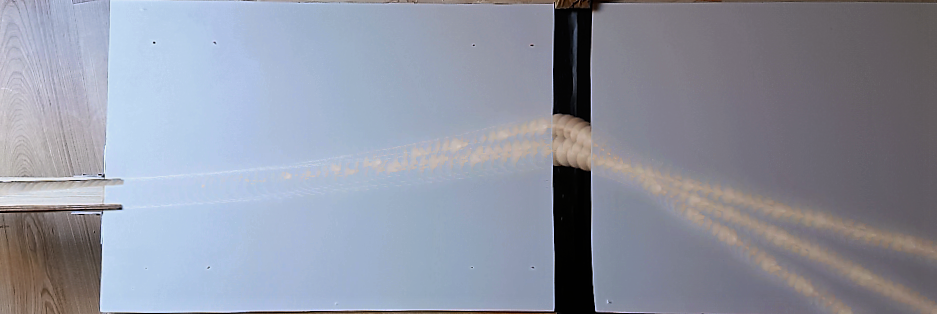
\includegraphics[width=0.99\textwidth]{images/aufbau2.png}
  \caption[Stroboskop-Effekt der Kugeln 8--10]{Die Bahnen der Kugeln 8--10 der Messreihe mit Kugeldurchmesser $r=\SI{35}{\milli\metre}$. Die Rampe befindet sich bei $y=\SI{0}{\centi\metre}$, die Düse des Gebläses bei $x=\SI{60}{\centi\metre}$ und $y=\SI{25}{\centi\metre}$.}
  \label{fig:aufbau2}
  \vspace{-0pt}
\end{figure}

\noindent Wie sich bei dem Vergleich mit \textsc{Mais} herausgestellt hat, werden nur gut $\SI{80}{\percent}$ der potentiellen in kinetische Energie umgesetzt. Um zu überprüfen, ob das neue Konzept für eine Beschleunigereinheit dazu in der Lage ist, die Energie signifikant besser umzuwandeln, wird neben den Daten aus Tabelle \ref{tab:energy} eine Messreihe mit der neuen Startvorrichtung aufgezeichnet, um anschließend einen \textit{Zweistichproben-Test} durchzuführen (siehe Abb. \ref{fig:aufbau2}).\footcite[vgl.][S.\,283]{Cramer2008} 

Bei der Messreihe werden $10$ Kugelbahnen (Radius $\SI{17.5}{\milli\metre}$) per Video aufgezeichnet. An der Beschleunigereinheit sind fünf Markierungen angebracht, von denen aus jeweils zwei Kugeln (1 und 6, 2 und 7 etc.) losgelassen werden. Ein Überblick der Messung liefert Tabelle \ref{tab:maisbex1}.

  \thisfloatsetup{
  capbesidewidth=\marginparwidth,
}
\begin{table}[htb]
\centering
%\sffamily,
\small
%\sansmath
\arrayrulecolor{white}
%\setlength{\arrayrulewidth}{2pt}
\vspace{0.2cm}
  \rowcolors{2}{halfgray!15}{halfgray!5}
 \setlength{\extrarowheight}{.00em}
			\begin{tabularx}{0.99\textwidth}{c*{1}{>{\RaggedLeft\arraybackslash}X}r*{2}{>{\RaggedLeft\arraybackslash}X}}		
\rowcolor{mycolor}  
\multicolumn{1}{c}{\color{white}\textbf{Kugel}} & 
\multicolumn{1}{c}{\color{white}\textbf{Höhe $\boldsymbol{h}$}} &
 \multicolumn{1}{c}{\color{white}\textbf{$\boldsymbol{E_\mathrm{pot}}$ in}} &  \multicolumn{1}{c}{\color{white}\textbf{$\boldsymbol{E_\mathrm{kin}}$ in}} &    \multicolumn{1}{c}{\color{white}\textbf{Abweichung}}\\ \rowcolor{mycolor}
 \multicolumn{1}{c}{\color{white}\textbf{Nr.}} & 
 \multicolumn{1}{c}{\color{white}\textbf{in $\boldsymbol{\si{\milli\metre}}$}} &
     \multicolumn{1}{c}{\color{white}\textbf{$\boldsymbol{\si{\milli\newton\metre}}$}}  &    \multicolumn{1}{c}{\color{white}\textbf{$\boldsymbol{\si{\milli\newton\metre}}$}}  &     \multicolumn{1}{c}{\color{white}\textbf{in $\si{\percent}$}}\\
1	&	22	&	3,392	&	3,050	&	10,1	\\
2	&	24	&	3,700	&	3,398	&	8,2	\\
3	&	35	&	5,396	&	5,242	&	2,8	\\
4	&	47	&	7,245	&	6,922	&	4,5	\\
5	&	60	&	9,250	&	8,813	&	4,7	\\
6	&	22	&	3,392	&	2,915	&	14,0	\\
7	&	24	&	3,700	&	3,398	&	8,2	\\
8	&	35	&	5,396	&	4,930	&	8,6	\\
9	&	47	&	7,245	&	6,706	&	7,4	\\
10	&	60	&	9,250	&	7,517	&	18,7	\\
		\end{tabularx}
		\caption[Umsetzung der potentiellen in kinetische Energie II]{Videoanalyse einer Messreihe mit Holzkugeln des Radius $r=\SI{17.5}{\milli\metre}$. Es werden die ersten $\SI{0.2}{\second}$ zur Berechnung der kinetischen Energie verwendet.}
		\label{tab:maisbex1}	
		\end{table} %\vspace*{-5cm}\newpage

\noindent Seien die beiden unabhängigen Stichproben normalverteilt mit dem Erwartungswert $\mu$ und der Varianz $\sigma^2$, d.\,h.
\begin{equation*}
X_1,...\,,X_{n_1}\distras{iid} N(\mu_1,\, \sigma^2),\,Y_1,\,,Y_{n_2}\distras{iid} Y(\mu_2,\, \sigma^2),
\end{equation*}
wobei angenommen wird, dass die Varianzen gleich sind, da die jeweiligen Startvorrichtungen aus dem gleichen Material erstellt wurden, so ergibt sich der Schätzer für die Varianz zu
\begin{equation*}
\widehat{\sigma}^2=\frac{1}{n_1+n_2-2}\left(\sum\limits_{i=1}^{n_1}(X_i-\overline{X})^2+\sum\limits_{j=1}^{n_2}(Y_j-\overline{Y})^2\right)\approx 18,49
\end{equation*}
Überprüft wird nun die \textit{Teststatistik} $\widehat{D}$
\begin{equation*}
=\frac{\overline{X}-\overline{Y}}{\widehat{\sigma}\sqrt{\sfrac{1}{n_1}+\sfrac{1}{n_2}}}\approx -6,84
\end{equation*}
mit der Entscheidungsregel \textit{die Nullhypothese $H_0: \mu_1\geq \mu_2$ wird abgelehnt, falls}
\begin{equation*}
\widehat{D}<-t_{1-\alpha}(n_1+n_2-2)
\end{equation*}
gilt, wobei $t_{1-\alpha}$ das Beta-Quantil der T-Verteilung ist \footnote{$\beta = 1-\alpha$}. Mit
\begin{equation*}
-t_{0,9995}(17)=-3,965 > \widehat{D}
\end{equation*}
kann zum Signifikanzniveau $\SI{99.95}{\percent}$ bewiesen werden, dass der Erwartungswert der Abweichung zwischen potentieller und kinetischer Energie geringer als bei der alten Startvorrichtung ist. 

Die Messungen der größten Holzkugeln haben im Mittel eine Umsetzung von $\SI{93}{\percent}$ der Lageenergie in kinetische Energie ergeben. Daher wird
das Funktionsprinzip der neuen Startvorrichtung als überlegen angesehen,
bei der mathematischen Beschreibung der Bewegungsgleichung $0,9\cdot E_\mathrm{pot}\approx \sfrac{7}{10}mv^2$ gesetzt und schließlich
vorgeschlagen, diese Beschleunigereinheit von der mechanischen Werkstatt anfertigen zu lassen. 

\section{Voraussagbarkeit}
\label{sec:voraus}
Im Zuge der Planung des Versuchsaufbaus wurde das erwartete Verhalten von Kugeln modelliert. Mit der im vorigen Abschnitt beschriebenen Messreihe wird nun überprüft, inwiefern das Modell Gültigkeit besitzt.

Für den Einfluss der schiefen Ebene werden die in Kapitel \ref{kap:4} aufgestellten Bewegungsgleichungen für die $x$- und $y$-Positionen der rollenden Massen verwendet. Die Krafteinwirkung des Strömungsfeldes wird zunächst als punktueller Kraftstoß angenommen, der eine Geschwindigkeitsänderung in $y$-Richtung verursacht. Damit ergeben sich die graphischen Auftragungen in Abbildung \ref{fig:plot1}

  \thisfloatsetup{%
  capbesidewidth=\marginparwidth}

\begin{figure}[htbp]
\centering
%\sansmath
\begin{tikzpicture}
\begin{axis}[	
	clip=false, % Verhindet weiße Punkte bei vielfach geplotteten x-Werten
	ymajorgrids,
    xmajorgrids,
          axis x line*=middle,
          axis y line*=center,
    grid style={white},
	axis on top,
    width=12cm,
    height=7.797cm,
    xmin=0,
    xmax=1200,
    ymin=-150,
    ymax=200,
    %/tikz/ybar interval,
    tick align=center,
    xtick align=outside,
    xlabel={$x$},
    ylabel={\rotatebox[origin=b]{270}{$y$}},   
   x label style={at={(axis cs:1000,-45)}},
    y label style={at={(axis cs:-150.5,150)}},
    axis line style={Honeydew4!70!black},
    ticklabel style={Honeydew4!70!black, inner sep=1pt,
                font=\footnotesize},
    yticklabels={${-150}$, ${-100}$, ${-50}$,  ${0}$,   ${50}$ , ${100}$, ${\si{\milli\newton}}$, ${200}$ },            
    xtick={200,400,600,800,1000, 1200},
    xticklabels={${200}$, ${400}$, ${600}$,  ${800}$, ${\si{\milli\metre}}$, ${1200}$},
     ytick={-150, -100, -50, 0, 50, 100,150,200 }, 
    scaled ticks=false,
    width=\textwidth,        
       legend style ={ at={(axis cs:150,-30)}, 
         anchor=north west, draw=none, 
             fill=none,align=left, text=Honeydew4!70!black,
              font=\footnotesize},                      
    cycle list name=mycolor4 white,                    
    label style={font=\small,Honeydew4!70!black,},
    enlarge x limits=true,
    %tick style={draw=none},
    x tick label as interval=false,
]
\draw[thick, Honeydew4!70!black, ->,>={latex[Honeydew4!70!black, round, length=0.4cm, width=4pt]}] (axis cs:-150.50, 110) -- (axis cs:-150.50, 190);
\draw[thick,Honeydew4!70!black, ->,>={latex[Honeydew4!70!black,round, length=0.4cm, width=4pt]}] (axis cs:900.00, -45) -- (axis cs:1100.00, -45);
\draw[thick, mycolor!50, fill=mycolor] (axis cs:675,18) circle (3pt);
\addplot
table[x = x, y =y]{images/data/10.dat};
\addlegendentry{$\SI{22.0}{\milli\metre}$};
\addplot
table[x = x, y =y]{images/data/11.dat};
\addlegendentry{$\SI{24.0}{\milli\metre}$};
\addplot
table[x = x, y =y]{images/data/12.dat};
\addlegendentry{$\SI{35.0}{\milli\metre}$};
\addplot
table[x = x, y =y]{images/data/13.dat};
\addlegendentry{$\SI{47.0}{\milli\metre}$};
\addplot
table[x = x, y =y]{images/data/14.dat};
\addlegendentry{$\SI{60.0}{\milli\metre}$};
\end{axis}
\clipright
\end{tikzpicture}
  \caption[Plot der theoretisch berechneten Kugelbahnen]{Plots der theoretisch berechneten Kugelbahnen für Starthöhen $h$, die mit denjenigen der Videoanalysen nahezu übereinstimmen. Der blaue Kreis deutet die approximative Fokussierungszone an (bei $(x,y)\tran = [(675, 19)\tran \pm (10 , 2)\tran] \si{\milli\metre}$).}
  \label{fig:plot1}
  \vspace{-0pt}
\end{figure}
  \thisfloatsetup{%
  capbesidewidth=\marginparwidth}

\begin{figure}[h!tb!p]
\centering
%\sansmath
\begin{tikzpicture}
\begin{axis}[	
	clip=false, % Verhindet weiße Punkte bei vielfach geplotteten x-Werten
	ymajorgrids,
    xmajorgrids,
          axis x line*=middle,
          axis y line*=center,
    grid style={white},
	axis on top,
    width=12cm,
    height=7.797cm,
    xmin=0,
    xmax=1200,
    ymin=-150,
    ymax=200,
    %/tikz/ybar interval,
    tick align=center,
    xtick align=outside,
    xlabel={$x$},
    ylabel={\rotatebox[origin=b]{270}{$y$}},   
   x label style={at={(axis cs:1000,-45)}},
    y label style={at={(axis cs:-150.5,150)}},
    axis line style={Honeydew4!70!black},
    ticklabel style={Honeydew4!70!black, inner sep=1pt,
                font=\footnotesize},
    yticklabels={${-150}$, ${-100}$, ${-50}$,  ${0}$,   ${50}$ , ${100}$, ${\si{\milli\newton}}$, ${200}$ },            
    xtick={200,400,600,800,1000, 1200},
    xticklabels={${200}$, ${400}$, ${600}$,  ${800}$, ${\si{\milli\metre}}$, ${1200}$},
     ytick={-150, -100, -50, 0, 50, 100,150,200 }, 
    scaled ticks=false,
    width=\textwidth,        
       legend style ={ at={(axis cs:150,-30)}, 
         anchor=north west, draw=none, 
             fill=none,align=left, text=Honeydew4!70!black,
              font=\footnotesize},                      
    cycle list name=mycolor4 black,                    
    label style={font=\small,Honeydew4!70!black,},
    enlarge x limits=true,
    %tick style={draw=none},
    x tick label as interval=false,
]
\draw[thick, Honeydew4!70!black, ->,>={latex[Honeydew4!70!black, round, length=0.4cm, width=4pt]}] (axis cs:-150.50, 110) -- (axis cs:-150.50, 190);
\draw[thick,Honeydew4!70!black, ->,>={latex[Honeydew4!70!black,round, length=0.4cm, width=4pt]}] (axis cs:900.00, -45) -- (axis cs:1100.00, -45);
\draw[thick, mycolor!50, fill=mycolor] (axis cs:700,20) circle (6pt);
\addplot
table[x = x, y =y]{images/data/15.dat};
\addlegendentry{$\SI{22.0}{\milli\metre}$};
\addplot
table[x = x, y =y]{images/data/16.dat};
\addlegendentry{$\SI{24.0}{\milli\metre}$};
\addplot
table[x = x, y =y]{images/data/17.dat};
\addlegendentry{$\SI{35.0}{\milli\metre}$};
\addplot
table[x = x, y =y]{images/data/18.dat};
\addlegendentry{$\SI{47.0}{\milli\metre}$};
\addplot
table[x = x, y =y]{images/data/19.dat};
\addlegendentry{$\SI{60.0}{\milli\metre}$};
\end{axis}
\clipright
\end{tikzpicture}
  \caption[Plot der gemessenen Kugelbahnen]{Plots der gemessenen Kugelbahnen für die Massen 6--10 mit den Starthöhen $h_i$. Der blaue Kreis deutet die ungefähre Fokussierungszone an (bei $(x,y)\tran = [(700, 20)\tran \pm (20 , 4)\tran] \si{\milli\metre}$).}
  \label{fig:plot2}
  \vspace{-40pt}
\end{figure}
\newpage

\noindent Die Kugeln 6--10 sind in Abbildung \ref{fig:plot2} aufgetragen. Die Fokussierungs-Zone liegt ca. $\SI{2.5}{\centi\metre}$ weiter als es bei den rechnerischen Werten der Fall ist, was sich mit den Erwartungen deckt: Die Impulsänderung erfolgt nach der Modellierung über eine Strecke von $\SI{6}{\centi\metre}$, d.\,h. drei Zentimeter vor $x=\SI{60}{\centi\metre}$ und drei dahinter. Über diese Distanz werden die Kugeln auf eine Kreisbahn gezwungen, wie dies auch im magnetischen Feld der Fall ist. Je schneller die Kugel, desto größer der Radius. Dadurch verschiebt sich die Spur der Kugeln im Mittel um die halbe Strecke des Kraftstoßes, d.\,h.  $\sfrac{6}{2}\,\si{\centi\metre}=\SI{3}{\centi\metre}$.

Die weiteren Messreihen mit Holzkugeln haben ähnliche, jedoch nicht so gute Ergebnisse geliefert. Die Fokussierung erfolgte jeweils im Bereich von $y=\SI{2}{\centi\metre}$ bis $\SI{5}{\centi\metre}$, wobei es zu mehr Fehlmessungen gekommen ist, die durch die Asymmetrie der Kugeln, mangelhafte Justierung der Startrampe und ein Hüpfen an dem Übergang zwischen den beiden Platten bedingt waren. Die Glasmurmeln lieferten keine akzeptablen Ergebnisse.

Bei dem endgültigen Versuchsaufbau sollten die Übergänge bis zu $\SI{5}{\centi\metre}$ abgeklebt werden, um die Höhendifferenz mit Acryl auszugleichen. Nach einer Antrockenzeit von einigen Stunden kann der gesamte Experimentiertisch beispielsweise mit Klavierlack ausgerollt werden, was den zusätzlichen Vorteil einer größeren Oberflächenhärte liefert, was den Rollwiderstand reduziert.

Die Verlässlichkeit ließe sich weiter erhöhen, indem industriell gefertigte Kugeln in Kugellagerqualität beschafft werden würden. Für einen Versuchsnachmittag sollte ein vollständiger Satz genügen.